\documentclass[a4paper]{jsbook}
\usepackage{take}

% ------------------- Title and Author -----------------------------
%\title{mining Package Documentation}
%\author{NYSOL}
\begin{document}

\begin{titlepage}
\begin{center}
{\huge Data Mining Package TAKE(竹) Documentation}\\
\vspace{10truept}
{\normalsize 対応 NYSOL パッケージ: Ver. 1.2,2.0}\\
\vspace{1cm}

revise history:\\

October 6, 2014 : mclque2g.rb,mbiclique.rbなどの追加、枝ファイル、節点ファイルの指定方法の変更\\
March 10, 2014 : nysol パッケージへの統合に伴いインストール方法変更\\
March 10, 2014 : mitemset.rb 改良,msequence.rb,mpolishing.rb など追加\\
February 28, 2014 : first release\\
\vspace{18cm}
{\small \today}

{\small Copyright \copyright 2013 by NYSOL CORPORATION}
\end{center}
\end{titlepage}

%\setlength{\baselineskip}{4mm}
\setcounter{tocdepth}{1}
%\label{mcmd:toc}
\tableofcontents

%\frontmatter
%\maketitle



\chapter{はじめに}
%\documentclass[a4paper]{book}
%\usepackage{zdd}
%\begin{document}

\section{Summary\label{sect:abstract}}
ZDD (Zero-suppressed Binary Decision Diagrams) is a data structure used for efficient manipulation of weighted item combinations based on reduction rules. ZDD VSOP (Valued-Sum-of-Products calculator)\cite{minato2005} is implemented as a Ruby Extension Library for the computation of item combinations. 

The founder of ZDD, Professor Shin-ichi Minato, developed a ZDD program which is made available for extended development in Ruby language. The Ruby Extension Library for ZDD is therefore developed in collaboration with \href{http://www-erato.ist.hokudai.ac.jp/index.php?language=jp}{ERATO Minato Discrete Structure Manipulation System Project}.

ZDD can enumerate huge number of combinations represented in a compact structure. For example, to enumerate all possible combinations of the products (frequent itemsets) purchased from the supermarket in the purchase history at a defined minimum support, in most cases, the number of combinations generated will grow exponentially. The ZDD data structure therefore is designed to provide a powerful framework to store all possible combinations in an unique and compact form efficiently.

Various calculations can be applied directly on ZDD objects where large scale itemsets are stored in a compact form for efficient processing.  
For example, users will be able to select the patterns containing "natto" from millions of enumerated frequent itemsets, or identify the differences of frequent itemset patterns between male and female. It is also possible to compute the ratio of size of ZDD. For details on theoretical context, please refer to \hyperref[sect:bib]{the reference} at the end of this document.

In this package, ZDD is handled as (known as {\bf ZDD object}) Ruby object.  Various functions for the ZDD objects correspond to class methods, operator overloading is used for ZDD objects using operands for ZDD object (\verb|+,-,==| etc.), to enable seamlessly integration of functions between Ruby and ZDD.

The ZDD package also supports automatic type conversion designed to reduce stress on   programming.

\section{Installation\label{sect:install}}
ZDD package is distributed as part of the mining package distribution by Nysol. Installation can be done by compiling from source or by installing rubygem.  Refer to mining package manual at \href{http://www.nysol.jp}{NYSOL} for details on the installation.

\section{Modify the maximum number of nodes}
The maximum number of ZDD nodes in this package is set to 40 million by default.
The program terminates with an error if the number of nodes exceeds this value.
The maximum number of nodes can be modified by setting the environment variable at \verb|ZDDLimitNode|.
For example, the maximum number of nodes can be set to 100 million nodes in the  bash shell as follows.
\begin{Verbatim}[baselinestretch=0.7,frame=single]
$ export ZDDLimitNode=100000000
\end{Verbatim}

The memory consumption per node is about 21-25 bytes on a 32bit OS machine. The program will consume about 1GB of main memory when the default limit of 40 million nodes is used. 

On a 64bit OS machine, the memory allocation is twice of the normal 32bit OS implementation, with 30\%percent increase in speed, and each node takes up to 28 to 32 bytes. Approximately 1.3GB of main memory is consumed when the program runs up to the default limit of 40 million nodes. By changing the maximum number of nodes according to the processing environment, the scale of ZDD structure can be increased.

\section{Terminologies\label{sect:terminology}}
The following section explains the terminologies used in this manual.
Note that there may be differences of the terms used in the \hyperref[sect:bib]{reference} at the end of this manual.

\subsubsection*{Item, Itemset, Term, Valued sum of products set, Expression}

An element in a set is referred to as "{\bf item}", and an "{\bf itemset}" contains a group of item elements.

The concept is easier to understand when these terms are set into context in a supermarket scenario. Commodity products are considered as items, and the combination of the products are referred to as itemset. When weight is attached to a "{\bf term}" in the itemset, it is known as "{\bf valued sum of products set}".
For example, the valued sum of products for 3 items a,b,c is represented as "\verb|abc+3ab+4bc+7c|" (this notation is referred to as "valued sum of products format"). It consists of four terms \verb|abc,3ab,4bc,7c|. In this case, \verb|3ab| consists of weight of \verb|3| for itemset \{a,b\}. Back to the supermarket scenario, this means that one customer purchased 3 products \verb|a,b,c| at the same time, and there are three customers who bought \verb|a,b| at the same time.

\subsubsection*{Empty itemset, ZDD constant object}
The itemset without element is referred to as "{\bf empty itemset}". Considering the valued sum of products set "\verb|abc+3ab+4bc+7c+3|", the a weight of \verb|3|  is attached to an empty itemset and thus it is shown as 3.

In supermarket scenario, it means that there are three customers did not purchase anything. 
Thus, empty itemsets of ZDD object is referred to as {\bf ZDD constant object}.

\subsubsection*{Item order table}
ZDD is a binary decision tree that contains a compact decision tree graph, and the level of the decision tree (depth) corresponds to the item. Further, this level, the order from  root to the leaves is managed by the table known as "{\bf item order table}".

It is important to manage item order since the order significantly impacts the size of ZDD (number of nodes). When the size of the ZDD increases, the processing speed will be reduced accordingly.
The item order table can be registered at any time using the \hyperref[sect:symbol]{symbol} function. If the number of combinations is extremely large, it is necessary to use the order table to register order of items.

\section{Notation\label{sect:notation}}

\subsubsection*{Notation of itemset}
The execution results in Ruby present the itemset which contains items and weight separated by space. Itemsets are displayed as character strings within text or comments, spaces between items are removed for simplicity.  For example, itemset \{a,b,c\} with weight of 3 is displayed as "\verb|3 a b c|" in the results. However, it will be displayed as "\verb|3abc|" in text or comment.

\subsubsection*{Example}

Multiple examples are included in this manual. The meaning of symbols used in the examples are as follows.\begin{itemize}
\item \verb|>| : Display Ruby input method.
\item \verb|$| : Display shell command line input.
\item \verb|#| : Display comments.
\item No symbol : Display the execution results.
\end{itemize}

The example contains the execution results log from the basic Ruby command line tool \verb|irb|. 


%\end{document}




\chapter{コマンド}

\section{mitemset.rb 頻出アイテム集合の列挙\label{sect:mitemset}}

トランザクションデータから頻出アイテム集合(頻出パターンとも呼ぶ)を列挙する。
列挙のコアアルゴリズムにはLCM(Linear time Closed itemset Miner)を用いている\cite{Uno2004,UnoWeb}。

本コマンドは以下のような特徴を持つ。
\begin{itemize}
 \item 他のアイテム集合に含まれないアイテム集合「極大アイテム集合」を列挙することができる。
 \item 同一の出現を持つ極大アイテム集合「飽和アイテム集合」を列挙することができる。
 \item アイテムの階層分類(taxonomy)を用いることができる。
 \item 分類クラスを指定することで、あるクラスに特徴的なパターン(顕在パターン:emerging patterns)を列挙することができる。
3つ以上のクラスにも対応している。
\end{itemize}

入力データとしては、表\ref{tbl:key},\ref{tbl:tra},\ref{tbl:matrix}で示される
ような多様なデータ型を用いることができるが、
本コマンドが直接扱うのはkey型データ(表\ref{tbl:key})のみである。
その他のデータ型は、MCMDパッケージの\verb|mtra|および\verb|mtraflg|コマンドによって、
あらかじめkey型データに変換しておく必要がある。

表\ref{tbl:key}において\verb|key|項目の値が同じ行、もしくは表\ref{tbl:tra},\ref{tbl:matrix}における各行のことを
特にトランザクションと呼び、トランザクションに含まれる要素をアイテムと呼ぶ。
スーパーマーケットの例では、トランザクションをレシート、アイテムを購入商品と考えればわかりやすいであろう。

\begin{table}[htbp]
\begin{center}
\begin{tabular}{ccc}

\begin{minipage}{0.3\hsize}
\begin{center}
\caption{key型データ\label{tbl:key}}
{\small
\begin{tabular}{cc}
\hline
key&item \\
\hline
T1&C \\
T1&E \\
T2&D \\
T2&E \\
T2&F \\
:&: \\ \hline
\end{tabular} 
}
\end{center}
\end{minipage}

\begin{minipage}{0.3\hsize}
\begin{center}
\caption{tra型データ\label{tbl:tra}}
{\small
\begin{tabular}{ll}
\hline
id&item \\
\hline
T1&C E \\
T2&D E F \\
T3&A B D F \\
T4&B D F \\
T5&A B D E \\
T6&A B D E F \\
\hline
\end{tabular} 
}
\end{center}
\end{minipage}

\begin{minipage}{0.3\hsize}
\begin{center}
\caption{行列型データ\label{tbl:matrix}}
{\small
\begin{tabular}{ccccccc}
\hline
id&A&B&C&D&E&F \\
\hline
T1& & &1& &1& \\
T2& & & &1&1&1\\
T3&1&1& &1& &1\\
T4& &1& &1& &1\\
T5&1&1& &1&1& \\
T6&1&1& &1&1&1\\
\hline
\end{tabular} 
}
\end{center}
\end{minipage}

\end{tabular} 
\end{center}
\end{table} 


\subsubsection{頻出アイテム集合}
頻出アイテム集合とは、出現頻度(サポートと呼ぶ)が
ユーザの与えた最小サポート以上であるようなアイテム集合のことを言う。
表\ref{tbl:tra}を例にとると、最小サポートが3件とすると、
アイテム集合\{B,D,F\}はT3,T5,T6の3件に出現しているので頻出であるが
アイテム集合\{B,D,E\}はT5,T6の2件にしか出現していないので頻出ではない。
ここで最小サポート3件を満たす頻出アイテム集合は、
\{A\},
\{A,B\},
\{A,B,D\},
\{A,D\},
\{B\},
\{B,D\},
\{B,D,F\},
\{B,F\},
\{D\},
\{D,E\},
\{D,F\},
\{E\},
\{F\}
の計13件である。

頻出アイテム集合を列挙すると、時にその数は膨大なものとなることがある。
そこで、列挙された頻出アイテム集合から代表的なアイテム集合のみを出力する
方法として、極大アイテム集合と飽和アイテム集合の列挙がある。

\subsubsection{極大アイテム集合}
ある頻出アイテム集合について、そのアイテム集合が
その他の頻出アイテム集合に包含されていなければ、
そのアイテム集合を頻出極大アイテム集合と呼ぶ。
前節に示してた13件の頻出アイテム集合のうち、\{A,B,D\},\{B,D,F\},\{D,E\}の3つのアイテム集合は、
他のどのアイテム集合にも包含されないので極大アイテム集合である。
その他のアイテム集合は、上記3つの極大アイテム集合のいずれかに包含されているため
極大ではない。

\subsubsection{飽和アイテム集合}
任意の二つの頻出アイテム集合について、
それらのアイテム集合が出現するトランザクションが同じであれば、
それら二つのアイテム集合は同じグループに属すると考える。
このようにして頻出アイテム集合をグルーピングすると、
各グループには、そのサイズが最も大きいアイテム集合がただ一つあることが分かっている。
このような頻出アイテム集合を飽和アイテム集合と呼ぶ。
例えば、\{A\},\{A,B\},\{A,D\},\{A,B,D\}は全てT3,T5,T6のトランザクションに出現するので同一グループである。
そしてこの中で最もサイズの大きい\{A,B,D\}が飽和集合ととして出力され、\{A\},\{A,B\},\{A,D\}は出力されない。
全ての飽和集合を列挙すると表\ref{tbl:close}の通り7つ存在する。
飽和集合という代表的なアイテム集合を列挙することで列挙件数を大幅に減少できている。
%ただし、データによっては、飽和集合を列挙したとしても全く列挙件数が減少しない
%ことも有りうる。

\begin{table}[htbp]
\begin{center}

\caption{飽和アイテム集合\label{tbl:close}}
{\small
\begin{tabular}{lll}
\hline
飽和集合&出現トランザクション&グループ \\
\hline
\{A,B,D\} & T3,T5,T6       & \{A\},\{A,B\},\{A,D\},\{A,B,D\} \\
\{B,D\}   & T3,T4,T5,T6    & \{B\},\{B,D\}  \\
\{B,D,F\} & T3,T4,T6       & \{B,F\},\{B,D,F\} \\
\{D\}     & T2,T3,T4,T5,T6 & \{D\} \\
\{D,E\}   & T2,T5,T6       & \{D,E\}    \\
\{D,F\}   & T2,T3,T4,T6    & \{F\},\{D,F\} \\
\{E\}     & T1,T2,T5,T6    & \{E\} \\ \hline
\end{tabular} 
}

\end{center}
\end{table} 

\subsubsection{顕在パターン}
各トランザクションが属する「クラス」を導入し、あるクラスに特徴的なパターン(ここでは頻出アイテム集合)を列挙する。
ここで特徴的とは、あるクラスには多頻度で、他のクラスでは多頻度でないことである。
例えば、スーパーマーケットでは、男性と女性で購買されるアイテムの違いを識別したい時などに使われる。
顕在パターンについてのより詳細な定義は\hyperref[sect:ep]{資料1}を参照のこと。
クラスデータは、表\ref{tbl:class}のように、トランザクションデータにクラス項目を結合することで与える。
同じトランザクションキーを持つ行は同じクラス値が与えられなければならない。

\begin{table}[htbp]
\begin{center}
\caption{key型データ\label{tbl:class}}
{\small
\begin{tabular}{ccc}
\hline
key&item&class \\
\hline
T1&C&pos \\
T1&E&pos \\
T2&D&neg \\
T2&E&neg \\
T2&F&neg \\
:&: \\ \hline
\end{tabular}
}
\end{center}
\end{table}

\subsubsection{階層分類}
アイテムの階層分類を反映させることができる。
例えば、スーパーマーケットでは「◯◯牛乳500ml」というアイテムは
「牛乳」に分類され、「牛乳」は「乳製品」に分類され、
さらに「乳製品」は食品に分類される。
このような階層分類を導入することで、「◯◯牛乳500ml」は「果物」と
購入される頻度が多いといった、階層分類の異なるアイテム間の関係を見つけることが
できるかもしれない。
ただし、現行バージョンでは、階層は1段階のみ対応している。

内部で行われる処理は至ってシンプルで、アイテムと分類の対応関係(表\ref{tbl:map})を与え、
入力データ(表\ref{tbl:org})のアイテムに応じた分類アイテムを追加(表\ref{tbl:add})、もしくは置換(表\ref{tbl:rep})した後に、
頻出アイテム集合を求める。
ただし、冗長なアイテム集合は出力されない。
冗長なアイテム集合とは、親子関係にあるアイテムペアを含むようなアイテム集合である。
例えば、表\ref{tbl:add}においてアイテム集合\{A,X\}はT3,T5,T6の3件に出現するが、
アイテムXはアイテムAと親子関係にあるため、このようなパターンは出力されない。
なお、冗長なアイテム集合の削除にはnysolのZDDパッケージ(\url{http://www.nysol.sakura.ne.jp/zdd/jp/})を利用している。


\begin{table}[htbp]
\begin{center}
\begin{tabular}{ccc}

\begin{minipage}{0.25\hsize}
\begin{center}
\caption{元データ\label{tbl:org}}
{\small
\begin{tabular}{ll}
\hline
id&item \\
\hline
T1&C E \\
T2&D E F \\
T3&A B D F \\
T4&B D F \\
T5&A B D E \\
T6&A B D E F \\
\hline
\end{tabular} 
}
\end{center}
\end{minipage}

\begin{minipage}{0.25\hsize}
\begin{center}
\caption{item-分類対応表\label{tbl:map}}
{\small
\begin{tabular}{cc}
\hline
item&taxonomy \\
\hline
A&X \\
B&X \\
C&Y \\
D&Z \\
E&Z \\
F&Z \\ \hline
\end{tabular} 
}
\end{center}
\end{minipage}

\begin{minipage}{0.25\hsize}
\begin{center}
\caption{分類追加後データ\label{tbl:add}}
{\small
\begin{tabular}{ll}
\hline
id&item \\
\hline
T1&C E Y Z\\
T2&D E F Z \\
T3&A B D F X Z\\
T4&B D F Y Z\\
T5&A B D E X Z\\
T6&A B D E F X Z\\
\hline
\end{tabular} 
}
\end{center}
\end{minipage}

\begin{minipage}{0.25\hsize}
\begin{center}
\caption{分類置換後データ\label{tbl:rep}}
{\small
\begin{tabular}{ll}
\hline
id&item \\
\hline
T1&Y Z\\
T2&Z \\
T3&X Z\\
T4&Y Z\\
T5&X Z\\
T6&X Z\\
\hline
\end{tabular} 
}
\end{center}
\end{minipage}

\end{tabular} 
\end{center}
\end{table} 

\subsubsection{出力}
本コマンドが出力するデータは、大きく分けて2つあり、一つは、列挙されたパターンデータ(\verb|patterns.csv|)、
そして他方は、それらのパターンをどのトランザクションが含むかについての情報(\verb|tid_pats.csv|)である。
パターンデータは、顕在パターンの場合異なるCSV項目を出力する。
表\ref{tbl:pat}〜表\ref{tbl:ep_pat}にそれらのサンプルを示す。

\begin{table}[htbp]
\begin{center}
\begin{tabular}{cc}

\begin{minipage}{0.6\hsize}
\begin{center}
\caption{patterns.csvのデータ例\label{tbl:pat}。pid項目は一つのパターンを識別するためのIDで、
sizeはパターンとしてのアイテム集合を構成するアイテム数、countはそのパターンが出現したトランザクション数、
そしてtotalは全トランザクション数である。supportは出現確率で、count/totalで計算される。liftはリフト値で、
期待される出現確率に対する実出現確率の比である。
最後にpatternがアイテム集合で、アイテムは半角スペースで区切られている。}
{\small
\begin{tabular}{crrrrrl}
\hline
pid&size&count&total&support&lift&pattern\\
\hline
 1&1&5&6&0.8333333333&1&D\\
 7&2&4&6&0.6666666667&1.2&D F\\
 6&1&4&6&0.6666666667&1&F\\
 4&1&4&6&0.6666666667&1&E\\
 2&1&4&6&0.6666666667&1&B\\
 3&2&4&6&0.6666666667&1.2&B D\\
 8&2&3&6&0.5&1.125&B F\\
 13&2&3&6&0.5&1.2&A D\\
\hline
\end{tabular} 
}
\\
{\small
アイテム集合$I=\{i_1,i_2,\cdots,i_n\}$のリフト値lift($I$)は次の通り定義される。
lift($I$)$=\frac{\Pr(I)}{\prod_{k=1}^n \Pr(i_k)}$
}
\end{center}
\end{minipage}
\begin{minipage}{0.3\hsize}
\begin{center}
\caption{tidpats.csvの内容例\label{tbl:tid_pats}。tidはトランザクションIDで、
tid=パラメータで指定した入力データ項目に対応している。
そしてそれぞれのトランザクションに含まれるパターンのIDがpidで示されている。
}
{\small
\begin{tabular}{cr}
\hline
tid&pid \\
\hline
 T1&4\\
 T2&1\\
 T2&4\\
 T2&7\\
 T2&6\\
 T2&5\\
 T3&10\\
 T3&6\\
\hline
\end{tabular} 
}
\end{center}
\end{minipage}

\end{tabular} 
\end{center}
\end{table} 

\begin{table}[htbp]
\begin{center}
\caption{顕在パターンにおけるpatterns.csvの内容例\label{tbl:ep_pat}。
class項目は、どのクラスに特徴的な顕在パターンか、その対象クラスを示している。
pid,pattern,size,totalは表\ref{tbl:pat}と同様である。
posは対象クラスのトランザクションに出現した件数で、
negはそれ以外のクラスのトランザクションに出現した件数である。
posTotal,negTotalは、対象クラスとそれ以外のクラスのトランザクション件数である。
supportは、対象クラスにおける出現確率で、pos/posTotalで計算される。
growthRateは増加率で、support/(neg/negTotal)で計算される値である。
分母が0の場合はinfと表示される。
この値が大きいほど、対象クラスに特徴的であることを意味する。
postProbは、パターンを条件とした時の対象クラスの事後確率で、
growthRateと同様、この値が大きいほど対象クラスに特徴的であることを意味する。
詳細な定義は\hyperref[sect:ep]{資料1}を参照のこと。
}
{\small
\begin{tabular}{cclrrrrrrrrr}
\hline
class&pid&pattern&size&pos&neg&posTotal&negTotal&total&support&growthRate&postProb\\
\hline
 cls2&13&A E&2&2&0&2&4&6&1&inf&1\\
 cls2&15&A B E&3&2&0&2&4&6&1&inf&1\\
 cls2&10&A B D E&4&2&0&2&4&6&1&inf&1\\
 cls2&14&B E&2&2&0&2&4&6&1&inf&1\\
 cls2&17&A D E&3&2&0&2&4&6&1&inf&1\\
 cls2&18&B D E&3&2&0&2&4&6&1&inf&1\\
 cls2&12&A B D&3&2&1&2&4&6&1&4&0.6666666667\\
 cls2&11&A D&2&2&1&2&4&6&1&4&0.6666666667\\
 cls2&16&D E&2&2&1&2&4&6&1&4&0.6666666667\\
\hline
\end{tabular} 
}
\end{center}
\end{table} 

% 上記項目の説明
% pid: パターン (アイテム集合)ID
% count: 出現件数 (トランザクション数)
% total: 全トランザクション数
% support: 出現確率 (=count/total)
% pattern: アイテム集合 (スペース区切り)

\subsection{書式}
\begin{verbatim}
mitemset.rb i= [x=] [O=] [tid=] [item=] [class=] [taxo=] [s=|S=] [sx=|SX=] [l=] [u=]
            [p=] [g=] [top=] [T=] [--help]

  i=       key型トランザクションデータファイル名【必須】
  c=       クラスファイル名【オプション】
  x=       階層分類データファイル名【オプション】
  O=       出力パス名【オプション:default=./take_#{日付時刻}】
  tid=     トランザクションID項目名【必須】
  item=    アイテム項目名(i=,x=上の項目名)【オプション:default="item"】
  class=   クラス項目名(c=上の項目名)【オプション】
           クラス項目名を指定すると顕在パターンが列挙される。
  taxo=    分類項目名【条件付き必須:x=】
  type=    アイテム集合のタイプ【オプション: default=F】
           F:頻出アイテム集合, C:飽和アイテム集合, M:極大アイテム集合
  s=       最小サポート(確率)【選択必須:s=, S=】
  S=       最小サポート(件数)【選択必須:s=, S=】
  sx=      最大サポート(確率)【オプション】
  SX=      最大サポート(件数)【オプション】
  l=       最小アイテム集合サイズ【オプション】
  u=       最大アイテム集合サイズ【オプション】
  p=       顕在パターン用最小事後確率【オプション:default=0.5】
  g=       顕在パターン用最小増加率【オプション】
  top=     列挙するパターン数の上限【オプション:default:制限なし】
  T=       ワークディレクトリ【オプション】
  --help   ヘルプの表示
\end{verbatim}

%\subsection*{備考}
%本コマンドで使われている列挙のコアアルゴリズムにはLCM(Linear time Closed itemset Miner)を用いている。
%詳細は以下の文献およびWebページを参照されたい。
%\begin{itemize}
%\item  Takeaki Uno, Tatsuya Asai, Yuzo Uchida, Hiroki Arimura, "An Efficient Algorithm for Enumerating Closed Patterns in Transaction Databases", Discovery Science 2004, LNAI 3245, pp.16-31.
%\item http://research.nii.ac.jp/~uno/codes-j.htm
%\end{itemize}

\subsection{利用例}
\subsubsection*{Example 1: Basic Example}

Enumerate frequent itemset that appear more than 3 times.


\begin{Verbatim}[baselinestretch=0.7,frame=single]
$ more dat1.csv
tid,item
T1,C
T1,E
T2,D
T2,E
T2,F
T3,A
T3,B
T3,D
T3,F
T4,B
T4,D
T4,F
T5,A
T5,B
T5,D
T5,E
T6,A
T6,B
T6,D
T6,E
T6,F
$ mitemset.rb  S=3 tid=tid item=item i=dat1.csv O=result1
#MSG# lcm_20140215 FIf /tmp/__MTEMP_18926_70182748393500_0 3 /tmp/__MTEMP_18926_7018274838
9080_0
trsact: /tmp/__MTEMP_18926_70182748393500_0 ,#transactions 6 ,#items 6 ,size 21 extracted 
database: #transactions 6 ,#items 5 ,size 20
 output to: /tmp/__MTEMP_18926_70182748389080_0
separated at 0
iters=8
14
1
5
6
2
trsact: /tmp/__MTEMP_18926_70182748393500_0 ,#transactions 6 ,#items 6 ,size 21 extracted 
database: #transactions 6 ,#items 6 ,size 21
 output to: /tmp/__MTEMP_18926_70182748389080_1
separated at 0
iters=7
6
0
6
#MSG# output patterns to CSV file ...
#MSG# the number of patterns enumerated is 13
#MSG# output tid-patterns ...
#MSG# The final results are in the directory `result1'
#END# /Users/stephane/.rvm/rubies/ruby-1.9.3-p448/bin/mitemset.rb S=3 tid=tid item=item i=
dat1.csv O=result1
$ more result1/patterns.csv
pid,size,count,total,support,lift,pattern
1,1,5,6,0.8333333333,1,D
7,2,4,6,0.6666666667,1.2,D F
6,1,4,6,0.6666666667,1,F
4,1,4,6,0.6666666667,1,E
2,1,4,6,0.6666666667,1,B
3,2,4,6,0.6666666667,1.2,B D
8,2,3,6,0.5,1.125,B F
13,2,3,6,0.5,1.2,A D
5,2,3,6,0.5,0.9,D E
12,3,3,6,0.5,1.8,A B D
11,2,3,6,0.5,1.5,A B
10,1,3,6,0.5,1,A
9,3,3,6,0.5,1.35,B D F
$ more result1/tid_pats.csv
tid,pid
T1,4
T2,1
T2,4
T2,7
T2,6
T2,5
T3,10
T3,6
T3,13
T3,7
T3,11
T3,8
T3,3
T3,12
T3,1
T3,2
T3,9
T4,6
T4,7
T4,8
T4,2
T4,1
T4,3
T4,9
T5,11
T5,13
T5,3
T5,1
T5,4
T5,10
T5,5
T5,2
T5,12
T6,2
T6,11
T6,6
T6,7
T6,5
T6,10
T6,1
T6,8
T6,12
T6,4
T6,9
T6,13
T6,3
\end{Verbatim}
\subsubsection*{Example 2: Set a limit on the size of itemset}

For itemsets that appear more than 3 or more times, patterns of itemsets with size 3 is enumerated.


\begin{Verbatim}[baselinestretch=0.7,frame=single]
$ mitemset.rb S=3 l=3 u=3 tid=tid item=item i=dat1.csv O=result2
#MSG# lcm_20140215 FIf -l 3 -u 3 /tmp/__MTEMP_19010_70360847449800_0 3 /tmp/__MTEMP_19010_
70360847467580_0
trsact: /tmp/__MTEMP_19010_70360847449800_0 ,#transactions 6 ,#items 6 ,size 21 extracted 
database: #transactions 6 ,#items 5 ,size 20
 output to: /tmp/__MTEMP_19010_70360847467580_0
separated at 0
iters=8
2
0
0
0
2
trsact: /tmp/__MTEMP_19010_70360847449800_0 ,#transactions 6 ,#items 6 ,size 21 extracted 
database: #transactions 6 ,#items 6 ,size 21
 output to: /tmp/__MTEMP_19010_70360847467580_1
separated at 0
iters=7
6
0
6
#MSG# output patterns to CSV file ...
#MSG# the number of patterns enumerated is 2
#MSG# output tid-patterns ...
#MSG# The final results are in the directory `result2'
#END# /Users/stephane/.rvm/rubies/ruby-1.9.3-p448/bin/mitemset.rb S=3 l=3 u=3 tid=tid item
=item i=dat1.csv O=result2
$ more result2/patterns.csv
pid,size,count,total,support,lift,pattern
0,3,3,6,0.5,1.35,B D F
1,3,3,6,0.5,1.8,A B D
\end{Verbatim}
\subsubsection*{Example 3: Enumerate closed itemsets}



\begin{Verbatim}[baselinestretch=0.7,frame=single]
$ mitemset.rb S=3 type=C tid=tid item=item i=dat1.csv O=result3
#MSG# lcm_20140215 CIf /tmp/__MTEMP_19093_70290667606020_0 3 /tmp/__MTEMP_19093_7029066760
1800_0
trsact: /tmp/__MTEMP_19093_70290667606020_0 ,#transactions 6 ,#items 6 ,size 21 extracted 
database: #transactions 6 ,#items 5 ,size 20
 output to: /tmp/__MTEMP_19093_70290667601800_0
separated at 0
iters=8
8
1
2
3
2
trsact: /tmp/__MTEMP_19093_70290667606020_0 ,#transactions 6 ,#items 6 ,size 21 extracted 
database: #transactions 6 ,#items 6 ,size 21
 output to: /tmp/__MTEMP_19093_70290667601800_1
separated at 0
iters=7
6
0
6
#MSG# output patterns to CSV file ...
#MSG# the number of patterns enumerated is 7
#MSG# output tid-patterns ...
#MSG# The final results are in the directory `result3'
#END# /Users/stephane/.rvm/rubies/ruby-1.9.3-p448/bin/mitemset.rb S=3 type=C tid=tid item=
item i=dat1.csv O=result3
$ more result3/patterns.csv
pid,size,count,total,support,lift,pattern
1,1,5,6,0.8333333333,1,D
2,2,4,6,0.6666666667,1.2,B D
3,1,4,6,0.6666666667,1,E
5,2,4,6,0.6666666667,1.2,D F
4,2,3,6,0.5,0.9,D E
6,3,3,6,0.5,1.35,B D F
7,3,3,6,0.5,1.8,A B D
\end{Verbatim}
\subsubsection*{Example 4: Enumerate maximal itemsets}



\begin{Verbatim}[baselinestretch=0.7,frame=single]
$ mitemset.rb S=3 type=M tid=tid item=item i=dat1.csv O=result4
#MSG# lcm_20140215 MIf /tmp/__MTEMP_19176_70274959882120_0 3 /tmp/__MTEMP_19176_7027495987
7480_0
trsact: /tmp/__MTEMP_19176_70274959882120_0 ,#transactions 6 ,#items 6 ,size 21 extracted 
database: #transactions 6 ,#items 5 ,size 20
 output to: /tmp/__MTEMP_19176_70274959877480_0
separated at 0
iters=8
3
0
0
1
2
trsact: /tmp/__MTEMP_19176_70274959882120_0 ,#transactions 6 ,#items 6 ,size 21 extracted 
database: #transactions 6 ,#items 6 ,size 21
 output to: /tmp/__MTEMP_19176_70274959877480_1
separated at 0
iters=7
6
0
6
#MSG# output patterns to CSV file ...
#MSG# the number of patterns enumerated is 3
#MSG# output tid-patterns ...
#MSG# The final results are in the directory `result4'
#END# /Users/stephane/.rvm/rubies/ruby-1.9.3-p448/bin/mitemset.rb S=3 type=M tid=tid item=
item i=dat1.csv O=result4
$ more result4/patterns.csv
pid,size,count,total,support,lift,pattern
0,2,3,6,0.5,0.9,D E
1,3,3,6,0.5,1.35,B D F
2,3,3,6,0.5,1.8,A B D
\end{Verbatim}
\subsubsection*{Example 5: Usage of hierarchical classification}



\begin{Verbatim}[baselinestretch=0.7,frame=single]
$ more taxo.csv
item,taxonomy
A,X
B,X
C,Y
D,Z
E,Z
F,Z
$ mitemset.rb S=4 tid=tid item=item i=dat1.csv x=taxo.csv taxo=taxonomy O=result5
#MSG# lcm_20140215 FIf /tmp/__MTEMP_19260_70240579278840_0 4 /tmp/__MTEMP_19260_7024057927
5400_0
trsact: /tmp/__MTEMP_19260_70240579278840_0 ,#transactions 6 ,#items 10 ,size 32 extracted
 database: #transactions 6 ,#items 6 ,size 27
 output to: /tmp/__MTEMP_19260_70240579275400_0
separated at 0
iters=6
22
1
6
9
5
1
trsact: /tmp/__MTEMP_19260_70240579278840_0 ,#transactions 6 ,#items 10 ,size 32 extracted
 database: #transactions 6 ,#items 9 ,size 32
 output to: /tmp/__MTEMP_19260_70240579275400_1
separated at 0
iters=9
9
0
9
#MSG# output patterns to CSV file ...
#MSG# reducing redundant rules in terms of taxonomy ...
#MSG# the number of patterns enumerated is 11
#MSG# output tid-patterns ...
#MSG# The final results are in the directory `result5'
#END# /Users/stephane/.rvm/rubies/ruby-1.9.3-p448/bin/mitemset.rb S=4 tid=tid item=item i=
dat1.csv x=taxo.csv taxo=taxonomy O=result5
$ more result5/patterns.csv
pid,size,count,total,support,lift,pattern
1,1,6,6,1,1,Z
2,1,5,6,0.8333333333,1,D
19,2,4,6,0.6666666667,1.2,D X
13,2,4,6,0.6666666667,1,B Z
14,1,4,6,0.6666666667,1,X
6,1,4,6,0.6666666667,1,F
11,2,4,6,0.6666666667,1.2,B D
21,2,4,6,0.6666666667,1,X Z
4,1,4,6,0.6666666667,1,E
10,1,4,6,0.6666666667,1,B
7,2,4,6,0.6666666667,1.2,D F
\end{Verbatim}
\subsubsection*{Example 6: Replace original items with hierarchical classification}



\begin{Verbatim}[baselinestretch=0.7,frame=single]
$ more taxo.csv
item,taxonomy
A,X
B,X
C,Y
D,Z
E,Z
F,Z
$ mitemset.rb S=4 tid=tid item=item i=dat1.csv x=taxo.csv taxo=taxonomy -replaceTaxo O=resul
t6
#MSG# lcm_20140215 FIf /tmp/__MTEMP_19394_70212028633240_0 4 /tmp/__MTEMP_19394_7021202864
5160_0
trsact: /tmp/__MTEMP_19394_70212028633240_0 ,#transactions 6 ,#items 4 ,size 11 extracted 
database: #transactions 6 ,#items 2 ,size 10
 output to: /tmp/__MTEMP_19394_70212028645160_0
separated at 0
iters=2
4
1
2
1
trsact: /tmp/__MTEMP_19394_70212028633240_0 ,#transactions 6 ,#items 4 ,size 11 extracted 
database: #transactions 6 ,#items 3 ,size 11
 output to: /tmp/__MTEMP_19394_70212028645160_1
separated at 0
iters=3
3
0
3
#MSG# output patterns to CSV file ...
#MSG# the number of patterns enumerated is 3
#MSG# output tid-patterns ...
#MSG# The final results are in the directory `result6'
#END# /Users/stephane/.rvm/rubies/ruby-1.9.3-p448/bin/mitemset.rb S=4 tid=tid item=item i=
dat1.csv x=taxo.csv taxo=taxonomy -replaceTaxo O=result6
$ more result6/patterns.csv
pid,size,count,total,support,lift,pattern
1,1,6,6,1,1,Z
2,1,4,6,0.6666666667,1,X
3,2,4,6,0.6666666667,1,X Z
\end{Verbatim}
\subsubsection*{Example 7: Enumerate emerging patterns}



\begin{Verbatim}[baselinestretch=0.7,frame=single]
$ more dat2.csv
tid,item,class
T1,C,cls1
T1,E,cls1
T2,D,cls1
T2,E,cls1
T2,F,cls1
T3,A,cls1
T3,B,cls1
T3,D,cls1
T3,F,cls1
T4,B,cls1
T4,D,cls1
T4,F,cls1
T5,A,cls2
T5,B,cls2
T5,D,cls2
T5,E,cls2
T6,A,cls2
T6,B,cls2
T6,D,cls2
T6,E,cls2
T6,F,cls2
$ mitemset.rb S=2 tid=tid item=item class=class i=dat2.csv p=0.6 O=result7
#MSG# lcm_20140215 FIA -w /tmp/__MTEMP_19510_70322251041060_1 /tmp/__MTEMP_19510_703222510
41060_0 1073741817 /tmp/__MTEMP_19510_70322251051500_0
trsact: /tmp/__MTEMP_19510_70322251041060_0 ,#transactions 6 ,#items 6 ,size 21 extracted 
database: #transactions 6 ,#items 4 ,size 17 ,weightfile /tmp/__MTEMP_19510_70322251041060
_1
 output to: /tmp/__MTEMP_19510_70322251051500_0
separated at 0
iters=6
9
1
4
3
1
#MSG# output patterns to CSV file ...
#MSG# the number of contrast patterns on class `cls1' enumerated is 8
#MSG# output tid-patterns ...
#MSG# lcm_20140215 FIA -w /tmp/__MTEMP_19510_70322251041060_2 /tmp/__MTEMP_19510_703222510
41060_0 2147483645 /tmp/__MTEMP_19510_70322251051500_2
trsact: /tmp/__MTEMP_19510_70322251041060_0 ,#transactions 6 ,#items 6 ,size 21 extracted 
database: #transactions 6 ,#items 4 ,size 16 ,weightfile /tmp/__MTEMP_19510_70322251041060
_2
 output to: /tmp/__MTEMP_19510_70322251051500_2
separated at 0
iters=14
11
0
1
5
4
1
#MSG# output patterns to CSV file ...
#MSG# the number of contrast patterns on class `cls2' enumerated is 11
#MSG# output tid-patterns ...
#MSG# the number of emerging patterns enumerated is 11
#MSG# The final results are in the directory `result7'
#END# /Users/stephane/.rvm/rubies/ruby-1.9.3-p448/bin/mitemset.rb S=2 tid=tid item=item cl
ass=class i=dat2.csv p=0.6 O=result7
$ more result7/patterns.csv
class,pid,pattern,size,pos,neg,posTotal,negTotal,total,support,growthRate,postProb
cls2,13,A E,2,2,0,2,4,6,1,inf,1
cls2,15,A B E,3,2,0,2,4,6,1,inf,1
cls2,10,A B D E,4,2,0,2,4,6,1,inf,1
cls2,14,B E,2,2,0,2,4,6,1,inf,1
cls2,17,A D E,3,2,0,2,4,6,1,inf,1
cls2,18,B D E,3,2,0,2,4,6,1,inf,1
cls2,12,A B D,3,2,1,2,4,6,1,4,0.6666666667
cls2,11,A D,2,2,1,2,4,6,1,4,0.6666666667
cls2,16,D E,2,2,1,2,4,6,1,4,0.6666666667
cls2,9,A B,2,2,1,2,4,6,1,4,0.6666666667
cls2,8,A,1,2,1,2,4,6,1,4,0.6666666667
\end{Verbatim}


\subsection{資料1: パラメータg=,p=,-uniformについて\label{sect:ep}}
クラス集合$C=\{c_1,c_2,\cdots,c_m\}$があり、各トランザクションは、いずれか一つのクラスに属しているものとする。
ここで我々が興味のある顕在パターンとは、ある対象クラスに頻出し、その他のクラスに頻出すしないようなアイテム集合である。
例えば、対象クラス$c_1$に頻出し、その他のクラス$c_2,c_3,\cdots,c_m$には頻出しないようなアイテム集合である。
以降、対象クラスを$c_t$、その他のクラスを$c_o$で表すものとする。

本コマンドでは顕在パターンを以下の3種類の方法により定義できる。
\begin{enumerate}
\item 増加率(クラス間の出現確率の比)の閾値を指定
\item 事後確率の閾値を指定(事前確率はデータ上の分布から推定)
\item 事後確率の閾値を指定(事前確率は各クラス一様)
\end{enumerate}

\subsubsection*{1.増加率}

対象クラス$c_t$におけるアイテム集合$I$の増加率$GR_t(I)$は式(\ref{gr})で表され、
対象クラスとその他クラスにおけるアイテム集合の出現確率の比として定義される。
そして、顕在パターンとは、ユーザが与えた最小増加率$\gamma$以上の増加率を持つようなアイテム集合のことである。
$\gamma$は、パラメータ\verb|g=|によって指定する。

\begin{equation}
GR_t(I)=\frac{\Pr(I|c_t)}{\Pr(I|c_o)} \ge \gamma \label{gr}
\end{equation}
%\begin{equation}
%GR_t(I) \ge \gamma \label{minGR}
%\end{equation}

\subsubsection*{2.事後確率}

%\item 事前確率は各クラス一様であると仮定した場合の、アイテム集合が観測後の対象クラスである事後確率がある閾値以上のアイテム集合
%\item アイテム集合が観測されたとき、対象クラスである事後確率がある閾値以上のアイテム集合

クラス未知のあるトランザクションについて、アイテム集合$I$を観測したとき、
そのトランザクションがクラス$c_t$に属する確率は、ベイズの定理より式(\ref{bayes})で表される。
この式は、クラス$c_t$の事前確率$\Pr(c_t)$がアイテム集合$I$を観測することで
事後確率$\Pr(c_t|I)$に更新されたことを意味する。
事前確率$\Pr(c_t)$は、与えられたデータにおけるクラス分布に基づいて推定する。
%すなわち、全トランザクション数に対するクラス$c_t$に属するトランザクションの割合である。
ここで、顕在パターンとは、ユーザが与えた最小事後確率$\pi$以上の事後確率を持つようなアイテム集合のことである。
$\pi$は、パラメータ\verb|p=|によって指定する。

\begin{equation}
\Pr(c_t|I)=\frac{\Pr(I|c_t)\Pr(c_t)}{\Pr(I|c_t)\Pr(c_t)+\Pr(I|c_o)\Pr(c_o)} \ge \pi \label{bayes}
%\Pr(c_t|I)=\frac{\Pr(I|c_t)}{\Pr(I)}\Pr(c_t) \ge \pi \label{bayes}
\end{equation}

\subsubsection*{3.事後確率(事前確率一様)}
全てのクラスの事前確率は一様であると仮定して上記の事後確率を計算する。
$\Pr(c_t)=\frac{1}{m}$,$\Pr(c_o)=\frac{m-1}{m}$を式(\ref{bayes})に代入すると式(\ref{bayes2})が得られる。
そして、顕在パターンとは、事前確率が一様であると仮定のもと、
ユーザが与えた最小事後確率$\pi_u$以上の事後確率を持つようなアイテム集合のことである。
$\pi_u$は、パラメータ\verb|p=|によって指定し、かつ\verb|-uniform|オプションを指定する。

\begin{equation}
%\Pr(c_t|I)=\frac{\Pr(I|c_t)\Pr(c_t)}{\Pr(I|c_t)\Pr(c_t)+\Pr(I|c_o)\Pr(c_o)} \label{bayes}
\Pr(c_t|I)=\frac{\Pr(I|c_t)}{\Pr(I|c_t)+(m-1)\Pr(I|c_o)} \ge \pi_{u} \label{bayes2}
\end{equation}

\subsubsection*{$GR_t(I)$と$Pr(c_t|I)$の関係}
式(\ref{gr})と式(\ref{bayes})より、$GR_t(I)$と$Pr(c_t|I)$の関係は式(\ref{relgrpost})で表される。
最小事後確率$\pi$を指定して顕在パターンを列挙する場合、
内部的には式(\ref{relgrpost})に従い、$\pi$を最小増加率$\gamma$に変換して実行している。

\begin{equation}
%\Pr(c_t|I)=\frac{\Pr(I|c_t)\Pr(c_t)}{\Pr(I|c_t)\Pr(c_t)+\Pr(I|c_o)\Pr(c_o)} \label{bayes}
GR_t(I)=\frac{\Pr(c_o)}{\Pr(c_t)}\cdot \frac{\Pr(c_t|I)}{1-\Pr(c_t|I)} \label{relgrpost}
\end{equation}

\subsection{資料2: LCMによる顕在パターン列挙について}

正例,負例のデータ集合をそれぞれ$D_t,D_o$とし,それらのサイズは$|D_t|=W |D_o|$の関係にあるとする.
いま,あるアイテム集合$I$(以下ではパターン$I$と呼ぶ)について,$D_t$における増加率$GR_t(I)$および出現ゲイン$Gain_t(I)$をそれぞれ式(\ref{gp}),(\ref{gain})の通り定義する.

\begin{equation}
GR_t(I)=\frac{sup(I,D_t)/|D_t|}{sup(I,D_o)/|D_o|}=W\frac{sup(I,D_t)}{sup(I,D_o)} \label{gp}
\end{equation}

\begin{equation}
%Gain_p(I)=\omega sup(I,D_t) /|D_t| - sup(I,D_o) /|D_o| \label{gain}
Gain_p(I)=\omega sup(I,D_t) - sup(I,D_o) \label{gain}
\end{equation}

ここで,$sup(I,D_t),sup(I,D_o)$はパターン$I$の$D_t,D_o$における出現件数で,
$\omega$は正例の出現数に与えるウェイトを表している.
パターン$I$について,$GR_t(I)$がユーザによって与えられた最小増加率
$\gamma$以上の場合,そのパターンを顕在パターンと呼び,
$Gain_p(I)$がユーザによって与えられた最小サポート$\sigma$以上の場合,
そのパターンをコントラストパターンと呼ぶことにする.
顕在パターンおよびコントラストパターンを正例,負例における
出現数の関係で示すと式(\ref{sup1}),(\ref{sup2})の通りとなる.

\begin{equation}
sup(I,D_o)\le \frac{W}{\gamma} sup(I,D_t) \label{sup1}
\end{equation}

\begin{equation}
sup(I,D_o)\le \omega sup(I,D_t) - \sigma \label{sup2}
\end{equation}

そして、負例における出現数$sup(I,D_o)$を$y$軸に,正例における出現数$sup(I,D_t)$を$x$軸としたとき,
顕在パターンは図\ref{fig:ep}の網かけで示された領域に属するパターンであり,
コントラストパターンは図\ref{fig:cp}の網かけで示された領域に属するパターンである.

\begin{figure}[htbp]
\begin{center}
\begin{tabular}{c}

\begin{minipage}{0.3\hsize}
\begin{center}
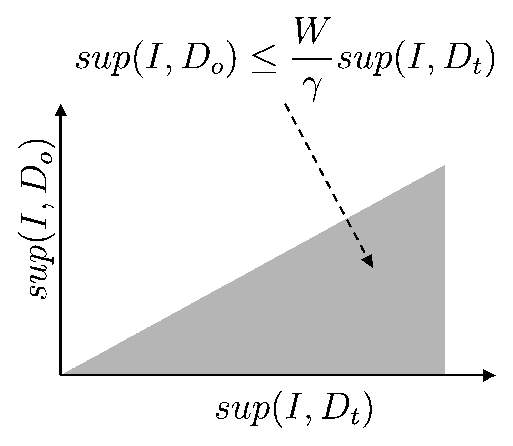
\includegraphics[scale=0.5]{./ep.eps}
\caption{顕在パターン\label{fig:ep}}
\end{center}
\end{minipage}

\begin{minipage}{0.3\hsize}
\begin{center}
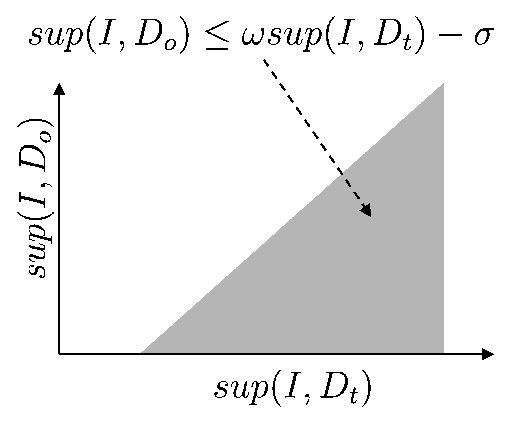
\includegraphics[scale=0.5]{./cp.eps}
\caption{コントラストパターン\label{fig:cp}}
\end{center}
\end{minipage}

\begin{minipage}{0.3\hsize}
\begin{center}
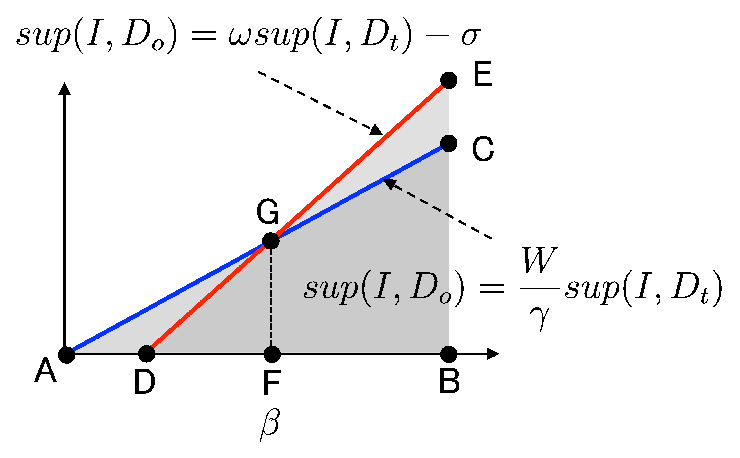
\includegraphics[scale=0.5]{./epcp.eps}
\caption{2つのパターンの関係\label{fig:epcp}}
\end{center}
\end{minipage}


\end{tabular} 
\end{center}
\end{figure} 

LCMでは,ユーザがパラメータ$\omega, \sigma$を与えることで
コントラストパターンを高速に列挙することができる.
コントラストパターンの列挙においては、$sup(I,D_t)$が大きくなればなるほど、
$sup(I,D_o)$との差が相対的に小さいパターンが列挙されることもあり、
そのようなパターンはクラス$c_t$に特徴的なパターンとは言えなくなる。
この欠点を回避するために、本コマンドでは顕在パターンの列挙を採用している。

ここで問題となるのは、コントラストパターンを列挙するLCMを使って、
いかに顕在パターンを列挙するかであり、以下に本コマンドで採用している方法を示す。

図\ref{fig:epcp}は、図\ref{fig:ep}と図\ref{fig:cp}を重ねた図である。
ここでは顕在パターンの領域ABCを全て列挙するのではなく、
$sup(I,D_t)\ge\beta$($\beta$は本コマンドS=で指定するパラメータ)を満たす領域GFCBに属する顕在パターンの列挙を考える。
LCMによって列挙されるパターンは、$\triangle{DEB}$に属するパターンであるが、
直線DEは、$\sigma$と$\omega$を定めることによって決まる。
まず$\sigma$は、直線ACと直線DEの交点Gの$x$座標が、ちょうど$\beta$になるように
設定する(式(\ref{sigma_beta}):$\omega$の決め方は後述)。
そうすることで、LCMが列挙した全パターンから、
$\triangle{DFG}$および$\triangle{EGC}$に属する
パターンを削除すれば、目的とする顕在パターンを列挙することが可能となる。

\begin{equation}
\sigma=\beta (\omega-\frac{W}{\gamma})  \label{sigma_beta}
\end{equation}



次に$\omega$であるが、これは直線DEの傾きを決めることに対応する。
一般的に$\triangle{EGC}$に属するパターンより、$\triangle{DGF}$に属するパターンの方が遥かに多いので、
$\omega$をできる限り大きくする方が効率的である。

しかしながら、$\omega$はトランザクションの重みであり、計算機上で件数をカウント
する変数の型の最大値に制約される。
その最大値を$maxInt$とすると、$\omega sup(I,D_t)\le maxInt$の制約を
満たしていなければならない。
$sup(I,D_t)$は$|D_p|$を超えることはないので、$\omega$を式(\ref{omega})のとおり
指定することで、$\triangle{DFG}$の列挙数を最小化できる。

\begin{equation}
\omega=\frac{maxInt}{|D_t|} \label{omega}
\end{equation}



\section{msequence.rb 頻出系列パターンの列挙\label{sect:msequence}}
アイテム系列データから頻出系列パターンを列挙する。
アイテム系列データとは、順序付けられたアイテム列の集合であり、
本コマンドは、アイテム系列データに多頻度に出現する部分系列をパターンとして列挙する。
系列パターンが系列データに出現(もしくはマッチ)するとは、
パターンを構成するアイテム全てが、その順序で系列データ上に現れることを意味する。
列挙のコアアルゴリズムにはLCMseq(LCM algorithm for enumerating all frequently appearing sequences)を用いている\cite{UnoWeb}。
本コマンドは以下のような特徴を持つ。
\begin{itemize}
% \item 他のパターンに含まれないパターン(極大パターン)を列挙することができる。
%\item 同一の出現件数における極大パターン(飽和パターン)を列挙することができる。
 \item gap長とwindow幅の制約条件(上限値)を与えることができる。
 \item gap長とwindow幅の制約条件(上限値)を時間制約として与えることも可能。
 \item アイテムの分類階層(taxonomy)を用いることができる。
 \item 分類クラスを指定することで、あるクラスに特徴的なパターン(顕在系列パターン)を列挙することができる。
3つ以上のクラスにも対応している。
 \item アイテム集合のシーケンス(同じ時刻に異なる複数のアイテム)は扱うことができない。
\end{itemize}

表\ref{tbl:seqDB}に、本コマンドが扱う入力データ例を示す。
tid項目によってひとつのシーケンスを識別し、time項目でitem項目の順序を表す。
同じ時刻に複数のitemを含めることはできない(
同時刻に複数のitemが存在した場合の動作は不定である)。
ただし、time項目は基本的にはitemの順序を決めるためのみに利用される。
\verb|-padding|オプションを指定した時のみ、整数で与えられたtime項目の値に応じたgap長やwindow幅の設定が可能となる(後述)。
また、表\ref{tbl:seqDB}のデータを、わかりやすさのためにアイテムの順序、及び時刻別の順序として表したデータを
、それぞれ表\ref{tbl:seqvDB}および表\ref{tbl:seqtimeDB}に示す。

\begin{table}[htbp]
\begin{center}
\begin{tabular}{ccc}

\begin{minipage}{0.2\hsize}
\begin{center}
\caption{系列データ\label{tbl:seqDB}}
{\small
\begin{tabular}{ccc}
\hline
tid&time&item\\
\hline
T1&0&C\\
T1&2&B\\
T1&3&A\\
T1&7&C\\
T2&2&D\\
  &:&\\
\hline
\end{tabular} 
}
\end{center}
\end{minipage}

\begin{minipage}{0.3\hsize}
\begin{center}
\caption{ベクトル型で表示\label{tbl:seqvDB}}
{\small
\begin{tabular}{cl}
\hline
  &シーケンス \\
\hline
T1&C B A C\\
T2&D A B C\\
T3&C B D E\\
T4&A C B\\
T5&B A D D C C\\
T6&A B D B C\\
\hline
\end{tabular} 
}
\end{center}
\end{minipage}

\begin{minipage}{0.5\hsize}
\begin{center}
\caption{時刻を考慮した表示\label{tbl:seqtimeDB}}
{\small
\begin{tabular}{ccccccccccc}
\hline
  &0&1&2&3&4&5&6&7&8&9 \\
\hline
T1&C& &B&A& & & &C& & \\
T2& & &D&A& &B&C& & & \\
T3& &C&B& &D& & & &E& \\
T4& & &A& & & &C& & &B\\
T5&B&A&D&D& & & &C& &C\\
T6&A& & & & &B&D& &B&C\\
\hline
\end{tabular} 
}
\end{center}
\end{minipage}

\end{tabular} 
\end{center}
\end{table} 

このデータについて2件以上出現する系列パターンは(A C),(B C),(D B C)など20件存在する(例1を参照)。
系列パターン(B C)は、tidがT1,T2,T5,T6のレコードに出現している。
T3、T4はアイテムBとCの両方を含んでいるが、出現順序が違うために出現したことにはならない。

%\subsubsection*{マッチとその位置}
%ここで系列パターンの出現について、より詳しく見ていく。
%系列パターンが系列データに出現(もしくはマッチ)するとは、
%パターンを構成するアイテム全てが、その順序でデータ上に出現することを意味する。
%また、後述するGAP制約およびWINDOW制約を理解するにあたって、
%パターンがデータ上でマッチする位置も重要である。
%例えば、パターン(B C)はデータ(B C C)に対して、1,2文字目にも、1,3文字目にもマッチするが、
%本コマンドでは前者のマッチを優先させる。
%そのルールは、パターンの各アイテムが最初にマッチした位置をマッチ位置とするものである。
%いくつかの例を表\ref{tbl:match}に示す。

%\begin{table}[htbp]
%\begin{center}
%\begin{tabular}{ccc}

%\begin{minipage}{0.4\hsize}
%\begin{center}
%\caption{パターン(A C)がマッチする位置。太字で示された位置にマッチしたことになる。\label{tbl:match}}
%{\small
%\begin{tabular}{l}
%\hline
%{\bf A}B{\bf C}D \\
%{\bf A}B{\bf C}CD \\
%B{\bf A}AB{\bf C}D \\
%{\bf A}AB{\bf C}CD \\
%{\bf A}BAB{\bf C}CD \\
%B{\bf A}AB{\bf C}ADC \\
%{\bf A}BCB{\bf C}D \\ \hline
%\end{tabular} 
%}
%\end{center}
%\end{minipage}
%\end{tabular} 
%\end{center}
%\end{table} 

\subsubsection*{頻出系列パターン}
頻出系列パターンとは、出現頻度(サポートと呼ぶ)が
ユーザの与えた最小サポート以上であるような系列パターンのことを言う。
最小サポートが3件とすると、
系列パターン(B D)は、系列データT3,T5,T6の3件に出現しているので頻出であるが
順序を逆にした系列パターン(D B)は、系列データT2,T6の2件にしか出現しないので頻出ではない。
%系列パターン(B D C)はT5,T6の2件にしか出現していないので頻出ではない。
ここで最小サポート3件を満たす全ての頻出系列パターンと、その出現件数を表\ref{tbl:freqSeq}に示す。

\begin{table}[htbp]
\begin{center}
\caption{表\ref{tbl:seqvDB}において最小サポート3件を満たす全頻出系列パターンとその出現トランザクション\label{tbl:freqSeq}}
\begin{tabular}{lcl}
\hline
系列パターン&出現件数&出現トランザクション \\
\hline
C   & 6 & T1,T2,T3,T4,T5,T6\\
B   & 6 & T1,T2,T3,T4,T5,T6\\
A   & 5 & T1,T2,T4,T5,T6 \\
A C & 5 & T1,T2,T4,T5,T6 \\
B C & 4 & T1,T2,T5,T6 \\
D   & 4 & T2,T3,T5,T6\\
A B & 3 & T2,T4,T6\\
B D & 3 & T3,T5,T6\\
C B & 3 & T1,T3,T4\\
D C & 3 & T2,T5,T6\\
\hline
\end{tabular} 
\end{center}
\end{table} 

%頻出アイテム集合を列挙すると、時にその数は膨大なものとなる。
%そこで、列挙された頻出系列パターンから代表的な系列パターンのみを出力する
%方法として、極大系列パターンの列挙がある。

%\subsubsection*{極大系列パターン}
%ある系列パターンが、その他の系列パターンに包含されていなければ(出現しなければ)、
%その系列パターンを極大系列パターンと呼ぶ。
%表\ref{tbl:freqSeq}において、(A B C)は他のどのパターンにも包含されていないので極大パターンであるが、
%(A),(B),(C),(A C),(B C),(A B)は、いずれも(A B C)に包含されているので極大ではない。
%極大系列パターンは、(B D),(C C),(A B C),(C B),(D C)の5つである。

\subsubsection*{顕在系列パターン}
各データが属する「クラス」を導入し、あるクラスに特徴的な系列パターンを列挙する。
ここで特徴的とは、あるクラスには多頻度で、他のクラスでは多頻度でないことである。
例えば、スーパーマーケットでは、男性と女性で購買されるアイテムの順序の違いを識別したい時などに使われる。
顕在系列パターンの列挙例は\hyperref[ex:ep1]{例5}を、
また、顕在系列パターンの評価指標として用いられる増加率や事後確率については、
\hyperref[sect:mitemset]{mitemset.rb}コマンドの\hyperref[sect:ep]{資料1}を参照のこと。

\subsubsection*{階層分類}
アイテムの階層分類を反映させることができる。
詳細は\hyperref[sect:mitemset]{mitemset.rb}コマンドを参照のこと。

\subsubsection*{gap長上限}
%列挙する系列パターンの系列データへのマッチの判定条件を制約することでができる。
%そのことにより、同じパターンであっても出現数が異なってくるため、
%結果として異なるパターンが列挙されることになる。
gap長とは、系列パターンの隣接する任意の2アイテムについて、
系列データ上でマッチした部分系列の距離(2アイテム間のアイテム数$-1$)として定義される。
例えば、系列パターン(A B C)と系列データ(A D D D B D C)では、
パターン上で隣接する2アイテムAB間の系列データ上でのgap長は4で、BC間のgap長は2である。
gap長上限を指定することによって、系列パターンの「出現」の定義を、パターン上の任意のgap長が指定した上限以下であるように制約する。
なお、複数のマッチが存在する場合は、いずれかのマッチが制約を満たしていれば出現したと考える。
gap長上限を1に設定すると、データ上で隣接する頻出系列パターンを列挙することになる。
gap長の計算例を表\ref{tbl:gapwin}に示す。

\subsubsection*{window幅上限}
window幅とは、マッチした系列データ上の部分系列について、その始点から終点までの長さ(アイテム数)である。
例えば、パターン(A B C)と系列データ(C A D C B D C)を考えると、
データ上のマッチした始点が2番目のアイテムで、終点が7番目目のアイテムとなり、window幅は6となる。
window幅上限を指定することによって、パターンの出現の定義を、データ上のマッチ幅が指定した上限以下であるように制約する。
なお、複数のマッチが存在する場合は、いずれかのマッチが制約を満たしていれば出現したと考える。
window幅の計算例を表\ref{tbl:gapwin}に示す。

\begin{table}[htbp]
\begin{center}
\caption{パターン(A B C)がマッチする位置と、そのgap長とwindow幅。
下の4行は、系列データAAABCCについて4通りのマッチが存在し、
それら全てのマッチについてのgap長とwindow幅を示している。
これらのgap長もしくはwindow幅の一つでも条件にマッチすれば出現したとみなされる。
例えば、window上限を3に設定した場合は、パターンABCは出現したことになるが、
上限を2にすると出現したことにはならない。
\label{tbl:gapwin}}
\begin{tabular}{lccc}
\hline
系列データ & A-B間gap長 & B-C間gap長 & window幅 \\
\hline
{\bf A} D D D D {\bf B} D {\bf C} D & 5 & 2 & 8 \\
{\bf A B C} D & 1 & 1 & 3 \\
C {\bf A} A C {\bf B} A {\bf C} C & 3 & 2 & 6\\
C {\bf A} C {\bf B} B A {\bf C} B C & 2 & 3 & 6\\
\hline
{\bf A} A {\bf B} {\bf C} C & 2 & 1 & 4\\
A {\bf A} {\bf B} {\bf C} C & 1 & 1 & 3\\
{\bf A} A {\bf B} C {\bf C} & 2 & 2 & 5\\
A {\bf A} {\bf B} C {\bf C} & 1 & 2 & 4\\
\hline
\end{tabular} 
\end{center}
\end{table} 

\subsubsection*{時間制約}
LCMseqでは、アイテムの出現時刻を直接指定してgap長制約やwindow幅制約を指定することができない。
そこで、前処理でアイテムが存在しない時刻に架空のアイテム("!":エクスクラメーションマーク)を導入することで時間制約を実現する。
\footnote{
そのため、アイテムの文字列として"!"を利用することはできない。
}
例えば、表\ref{tbl:seqtimeDB}に示された系列データは、表\ref{tbl:paddingDB}に示されるようなデータに変換される。
そして、架空アイテムを挿入した系列データに対してgap長制約やwindow制約を指定して系列パターンを列挙する。
そして最終の出力時に架空アイテムを含む系列パターンの出力を抑制する。

\begin{table}[htbp]
\begin{center}
\caption{時間を考慮したgap長制約とwindow制約を実現するために、アイテムの存在しない時刻に架空のアイテム"!"を挿入する。
\label{tbl:paddingDB}}
{\small
\begin{tabular}{cl}
\hline
  &シーケンス \\
\hline
T1&C ! B A ! ! ! C\\
T2&D A ! B C\\
T3&C B ! D ! ! ! E\\
T4&A ! ! ! C ! ! B\\
T5&B A D D ! ! ! C ! C\\
T6&A ! ! ! ! B D B ! C\\
\hline
\end{tabular} 
}
\end{center}
\end{table} 

\subsubsection{出力}
本コマンドが出力するデータは、大きく分けて2つあり、一つは、列挙された系列パターンデータ(\verb|patterns.csv|)、
そして他方は、それらのパターンをどのトランザクションが含むかについての情報(\verb|tid_pats.csv|である。
パターンデータは、顕在系列パターンの場合異なるCSV項目を出力する。
表\ref{tbl:qpat}〜表\ref{tbl:qep_pat}にそれらのサンプルを示す。

\begin{table}[htbp]
\begin{center}
\begin{tabular}{cc}

\begin{minipage}{0.6\hsize}
\begin{center}
\caption{patterns.csvのデータ例\label{tbl:qpat}。pid項目は一つの系列パターンを識別するためのIDで、
sizeはパターンとしてのアイテム集合を構成するアイテム数、countはそのパターンが出現した系列データ数、
そしてtotalは全系列データ数である。supportは出現確率で、count/totalで計算される。
最後にpatternが系列パターンで、アイテムは半角スペースで区切られている。}
{\small
\begin{tabular}{crrrrl}
\hline
pid&pattern&size&count&total&support \\
\hline
1  & C  &1&6&6&1\\
4  & B  &1&6&6&1\\
11 & A C&2&5&6&0.8333333333\\
10 & A  &1&5&6&0.8333333333\\
16 & D  &1&4&6&0.6666666667\\
7  & B C&2&4&6&0.6666666667\\
12 & A B&2&3&6&0.5\\
2  & C B&2&3&6&0.5\\
19 & D C&2&3&6&0.5\\
3  & C C&2&2&6&0.3333333333\\
:  & :  &:&:&:&:\\
\hline
\end{tabular} 
}
\end{center}
\end{minipage}

\begin{minipage}{0.35\hsize}
\begin{center}
\caption{tidpats.csvの内容例\label{tbl:qtid_pats}。tidは系列データIDで、
tid=パラメータで指定した入力データ項目に対応している。
そしてそれぞれの系列データに含まれる系列パターンのIDがpidで示されている。
}
{\small
\begin{tabular}{cr}
\hline
tid&pid \\
\hline
T1&0 \\
T1&1 \\
T1&10 \\
T1&2 \\
T2&0 \\
T2&1 \\
T2&10 \\
T2&11 \\
T3&0 \\
T3&1 \\
:&: \\
\hline
\end{tabular} 
}
\end{center}
\end{minipage}

\end{tabular} 
\end{center}
\end{table} 

\begin{table}[htbp]
\begin{center}
\caption{顕在パターンにおけるpatterns.csvの内容例\label{tbl:qep_pat}。
class項目は、どのクラスに特徴的な顕在パターンか、その対象クラスを示している。
pid,pattern,size,totalは表\ref{tbl:qpat}と同様である。
posは対象クラスのトランザクションに出現した件数で、
negはそれ以外のクラスのトランザクションに出現した件数である。
posTotal,negTotalは、対象クラスとそれ以外のクラスのトランザクション件数である。
supportは、対象クラスにおける出現確率で、pos/posTotalで計算される。
growthRateは増加率で、support/(neg/negTotal)で計算される値である。
分母が0の場合はinfと表示される。
この値が大きいほど、対象クラスに特徴的であることを意味する。
postProbは、パターンを条件とした時の対象クラスの事後確率で、
growthRateと同様、この値が大きいほど対象クラスに特徴的であることを意味する。
詳細な定義はmitemset.rbコマンドの解説の\hyperref[sect:ep]{資料1}を参照のこと。
}
{\small
\begin{tabular}{cclrrrrrrrrr}
\hline
class&pid&pattern&size&pos&neg&posTotal&negTotal&total&support&growthRate&postProb\\
\hline
cls1&1&B C&2&3&0&4&2&6&0.75&inf&1\\
cls2&9&B C D&3&2&0&2&4&6&1&inf&1\\
cls2&10&A D&2&2&0&2&4&6&1&inf&1\\
cls2&11&A C D&3&2&0&2&4&6&1&inf&1\\
cls2&8&B D&2&2&1&2&4&6&1&4&0.6666666667\\
cls2&12&C D&2&2&1&2&4&6&1&4&0.6666666667\\
\hline
\end{tabular} 
}
\end{center}
\end{table} 

\subsection{書式}
\begin{verbatim}
msequence.rb i= [x=] [O=] [tid=] [item=] [class=] [taxo=] [s=|S=] [sx=|SX=] [l=] [u=]
             [gap=] [win=] [p=] [g=] [top=] [-padding] [T=] [--help]

  i=       key型トランザクションデータファイル名【必須】
  c=       クラスファイル名【オプション】
  x=       階層分類データファイル名【オプション】
  O=       出力パス名【オプション:default=./take_#{日付時刻}】
  tid=     トランザクションID項目名【必須】
  time=    トランザクションID項目名【必須】
  item=    時間項目名(i=上の項目名)【オプション:default="time"】 
  class=   クラス項目名(c=上の項目名)【オプション】
           クラス項目名を指定すると顕在パターンが列挙される。
  taxo=    分類項目名【条件付き必須:x=】
  s=       最小サポート(確率)【選択必須:s=, S=】
  S=       最小サポート(件数)【選択必須:s=, S=】
  sx=      最大サポート(確率)【オプション】
  SX=      最大サポート(件数)【オプション】
  l=       最小アイテム集合サイズ【オプション】
  u=       最大アイテム集合サイズ【オプション】
  gap=     パターンのギャップ長の上限(0以上の整数)【オプション:0で制限無し,default:0】
  win=     パターンの窓サイズの上限(0以上の整数)【オプション:0で制限無し,default:0】
  p=       顕在パターン用最小事後確率【オプション:default=0.5】
  g=       顕在パターン用最小増加率【オプション】
  top=     列挙するパターン数の上限【オプション:default:制限なし】
  -padding 時刻を整数とみなし、連続でない時刻に特殊なアイテムがあることを想定する。
           gap=やwin=の指定に影響する。
  T=       ワークディレクトリ【オプション】
  --help   ヘルプの表示
\end{verbatim}

\subsection{利用例}
\subsubsection*{例1: 基本例}

2件以上で出現する系列パターン。
入力データの項目名は、全てデフォルトのものと同じなので省略していることに注意する。


\begin{Verbatim}[baselinestretch=0.7,frame=single]
$ more dat1.csv
tid,time,item
T1,0,C
T1,2,B
T1,3,A
T1,7,C
T2,2,D
T2,3,A
T2,5,B
T2,6,C
T3,1,C
T3,2,B
T3,4,D
T3,8,E
T4,2,A
T4,5,C
T4,6,B
T5,0,B
T5,1,A
T5,2,D
T5,3,D
T5,7,C
T5,9,C
T6,0,A
T6,5,B
T6,6,D
T6,8,B
T6,9,C
$ msequence.rb  O=result1 i=dat1.csv S=2
#MSG# lcm_seq_20140215 CIf /tmp/__MTEMP_96779_70117174398360_0 2 /tmp/__MTEMP_96779_701171
74386400_0
trsact: /tmp/__MTEMP_96779_70117174398360_0 ,#transactions 6 ,#items 5 ,size 26 extracted 
database: #transactions 6 ,#items 4 ,size 25
 output to: /tmp/__MTEMP_96779_70117174386400_0
iters=20
20
1
4
10
5
#MSG# output tid-patterns ...
#MSG# the number of contrast patterns enumerated is 19
#MSG# The final results are in the directory `result1'
#END# /usr/bin/msequence.rb O=result1 i=dat1.csv S=2
$ more result1/patterns.csv
pid,pattern,size,count,total,support
1,C,1,6,6,1
4,B,1,6,6,1
11,A C,2,5,6,0.8333333333
10,A,1,5,6,0.8333333333
16,D,1,4,6,0.6666666667
7,B C,2,4,6,0.6666666667
12,A B,2,3,6,0.5
8,B D,2,3,6,0.5
2,C B,2,3,6,0.5
19,D C,2,3,6,0.5
3,C C,2,2,6,0.3333333333
18,D B C,3,2,6,0.3333333333
13,A B C,3,2,6,0.3333333333
14,A D,2,2,6,0.3333333333
15,A D C,3,2,6,0.3333333333
9,B D C,3,2,6,0.3333333333
17,D B,2,2,6,0.3333333333
6,B A C,3,2,6,0.3333333333
5,B A,2,2,6,0.3333333333
\end{Verbatim}
\subsubsection*{例2: パターン長の制限}

出現頻度が3以上の長さが2の系列パターンのみを列挙する。


\begin{Verbatim}[baselinestretch=0.7,frame=single]
$ msequence.rb  O=result2 i=dat1.csv S=3 l=2 u=2
#MSG# lcm_seq_20140215 CIf -l 2 -u 2 /tmp/__MTEMP_96838_70227485417240_0 3 /tmp/__MTEMP_96
838_70227485416360_0
trsact: /tmp/__MTEMP_96838_70227485417240_0 ,#transactions 6 ,#items 5 ,size 26 extracted 
database: #transactions 6 ,#items 4 ,size 25
 output to: /tmp/__MTEMP_96838_70227485416360_0
iters=11
6
0
0
6
#MSG# output tid-patterns ...
#MSG# the number of contrast patterns enumerated is 6
#MSG# The final results are in the directory `result2'
#END# /usr/bin/msequence.rb O=result2 i=dat1.csv S=3 l=2 u=2
$ more result2/patterns.csv
pid,pattern,size,count,total,support
3,A C,2,5,6,0.8333333333
1,B C,2,4,6,0.6666666667
0,C B,2,3,6,0.5
2,B D,2,3,6,0.5
4,A B,2,3,6,0.5
5,D C,2,3,6,0.5
$ more result2/tid_pats.csv
tid,pid
T1,0
T1,1
T1,3
T2,1
T2,3
T2,4
T2,5
T3,0
T3,2
T4,0
T4,3
T4,4
T5,1
T5,2
T5,3
T5,5
T6,1
T6,2
T6,3
T6,4
T6,5
\end{Verbatim}
\subsubsection*{例3: gap長とwindowサイズの指定}

出現頻度が2以上、長さが2以上の系列パターンのうち、gap長が2、windowサイズが4のパターンを列挙する。


\begin{Verbatim}[baselinestretch=0.7,frame=single]
$ msequence.rb  O=result3 i=dat1.csv S=2 l=2 gap=2 win=4
#MSG# lcm_seq_20140215 CIf -l 2 -g 2 -G 4 /tmp/__MTEMP_96898_70310565879140_0 2 /tmp/__MTE
MP_96898_70310565878100_0
trsact: /tmp/__MTEMP_96898_70310565879140_0 ,#transactions 6 ,#items 5 ,size 26 extracted 
database: #transactions 6 ,#items 5 ,size 26
 output to: /tmp/__MTEMP_96898_70310565878100_0
iters=15
10
0
0
9
1
#MSG# output tid-patterns ...
#MSG# the number of contrast patterns enumerated is 10
#MSG# The final results are in the directory `result3'
#END# /usr/bin/msequence.rb O=result3 i=dat1.csv S=2 l=2 gap=2 win=4
$ more result3/patterns.csv
pid,pattern,size,count,total,support
0,C B,2,3,6,0.5
2,B C,2,3,6,0.5
3,B D,2,3,6,0.5
4,A C,2,3,6,0.5
5,A B,2,3,6,0.5
1,B A,2,2,6,0.3333333333
6,A D,2,2,6,0.3333333333
7,D B,2,2,6,0.3333333333
8,D B C,3,2,6,0.3333333333
9,D C,2,2,6,0.3333333333
\end{Verbatim}
\subsubsection*{例4: paddingにより時刻を考慮する}

例3と同じ条件で、-paddingを指定することで、時間を考慮したgap長とwindowサイズ制約により系列パターンを列挙する。


\begin{Verbatim}[baselinestretch=0.7,frame=single]
$ msequence.rb  O=result4 i=dat1.csv S=2 l=2 gap=2 win=4 -padding
#MSG# lcm_seq_zero_20140215 CIf -l 2 -g 2 -G 4 /tmp/__MTEMP_96957_70107510988120_0 2 /tmp/
__MTEMP_96957_70107510987120_0
trsact: /tmp/__MTEMP_96957_70107510988120_0 ,#transactions 6 ,#items 6 ,size 46 extracted 
database: #transactions 6 ,#items 6 ,size 46
 output to: /tmp/__MTEMP_96957_70107510987120_0
iters=33
4
0
0
4
#MSG# output tid-patterns ...
#MSG# the number of contrast patterns enumerated is 4
#MSG# The final results are in the directory `result4'
#END# /usr/bin/msequence.rb O=result4 i=dat1.csv S=2 l=2 gap=2 win=4 -padding
$ more result4/patterns.csv
pid,pattern,size,count,total,support
0,C B,2,3,6,0.5
3,B D,2,3,6,0.5
1,B A,2,2,6,0.3333333333
2,B C,2,2,6,0.3333333333
\end{Verbatim}
\subsubsection*{例5: 顕在系列パターンの列挙\label{ex:ep1}}

例1と同じ条件で、クラス項目を指定することで顕在パターンを列挙する。


\begin{Verbatim}[baselinestretch=0.7,frame=single]
$ more dat2.csv
tid,time,item,class
T1,0,C,cls1
T1,2,B,cls1
T1,3,A,cls1
T1,7,C,cls1
T2,2,D,cls1
T2,3,A,cls1
T2,5,B,cls1
T2,6,C,cls1
T3,1,C,cls1
T3,2,B,cls1
T3,4,D,cls1
T3,8,E,cls1
T4,2,A,cls1
T4,5,C,cls1
T4,6,B,cls1
T5,0,B,cls2
T5,1,A,cls2
T5,2,D,cls2
T5,3,D,cls2
T5,7,C,cls2
T5,9,C,cls2
T6,0,A,cls2
T6,5,B,cls2
T6,6,D,cls2
T6,8,B,cls2
T6,9,C,cls2
$ msequence.rb  O=result5 i=dat2.csv S=2 class=class -padding
#MSG# lcm_seq_zero_20140215 CIA -w /tmp/__MTEMP_97018_70131049887220_1 /tmp/__MTEMP_97018_
70131049887220_0 1073741815 /tmp/__MTEMP_97018_70131049885920_0
trsact: /tmp/__MTEMP_97018_70131049887220_0 ,#transactions 6 ,#items 6 ,size 46 extracted 
database: #transactions 6 ,#items 5 ,size 45 ,weightfile /tmp/__MTEMP_97018_70131049887220
_1
 output to: /tmp/__MTEMP_97018_70131049885920_0
iters=33
9
1
4
4
#MSG# output patterns to CSV file ...
#MSG# the number of contrast patterns on class `cls1' enumerated is 8
#MSG# output tid-patterns ...
#MSG# lcm_seq_zero_20140215 CIA -w /tmp/__MTEMP_97018_70131049887220_2 /tmp/__MTEMP_97018_
70131049887220_0 2147483645 /tmp/__MTEMP_97018_70131049885920_2
trsact: /tmp/__MTEMP_97018_70131049887220_0 ,#transactions 6 ,#items 6 ,size 46 extracted 
database: #transactions 6 ,#items 5 ,size 45 ,weightfile /tmp/__MTEMP_97018_70131049887220
_2
 output to: /tmp/__MTEMP_97018_70131049885920_2
iters=36
5
0
0
3
2
#MSG# output patterns to CSV file ...
#MSG# the number of contrast patterns on class `cls2' enumerated is 5
#MSG# output tid-patterns ...
#MSG# the number of emerging sequence patterns enumerated is 13
#MSG# The final results are in the directory `result5'
#END# /usr/bin/msequence.rb O=result5 i=dat2.csv S=2 class=class -padding
$ more result5/patterns.csv
class,pid,pattern,size,pos,neg,posTotal,negTotal,total,support,growthRate,postProb
cls1,1,B C,2,3,0,4,2,6,0.75,inf,1
cls2,10,A D,2,2,0,2,4,6,1,inf,1
cls2,9,B C D,3,2,0,2,4,6,1,inf,1
cls2,11,A C D,3,2,0,2,4,6,1,inf,1
cls1,0,C,1,4,2,4,2,6,1,1,0.6666666667
cls1,2,B,1,4,2,4,2,6,1,1,0.6666666667
cls1,6,A B,2,2,1,4,2,6,0.5,1,0.6666666667
cls2,8,B D,2,2,1,2,4,6,1,4,0.6666666667
cls2,12,C D,2,2,1,2,4,6,1,4,0.6666666667
cls1,5,A C,2,3,2,4,2,6,0.75,0.75,0.6
cls1,4,A,1,3,2,4,2,6,0.75,0.75,0.6
cls1,7,D,1,2,2,4,2,6,0.5,0.5,0.5
cls1,3,B C,2,2,2,4,2,6,0.5,0.5,0.5
\end{Verbatim}





\section{mpolishing.rb 一般グラフの研磨\label{sect:mpolishing}}

一般グラフデータに対して、データ研磨アルゴリズムを適用することで、
ノイズを除去し、グラフの濃淡をより鮮明にした「研磨グラフ」を生成する。
まずは、直感的な理解を得るために、図\ref{fig:polish0}と図\ref{fig:polish1}に研磨前のグラフと研磨後のグラフを示す。
オリジナルのグラフについて、濃い部分構造はより濃く、そして薄い部分構造はより薄くなるように研磨される。
結果として、中規模の極大クリーク(他の完全部分グラフに包含されない完全部分グラフ)が多く生成される。

\begin{figure}[htbp]
\begin{center}
\begin{tabular}{cc}

\begin{minipage}{0.3\hsize}
\begin{center}
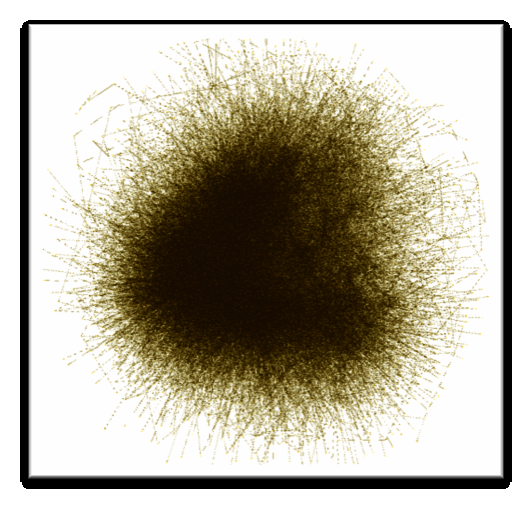
\includegraphics[scale=0.5]{./polish0.eps}
\caption{研磨前のグラフ\label{fig:polish0}}
\end{center}
\end{minipage}

\begin{minipage}{0.3\hsize}
\begin{center}
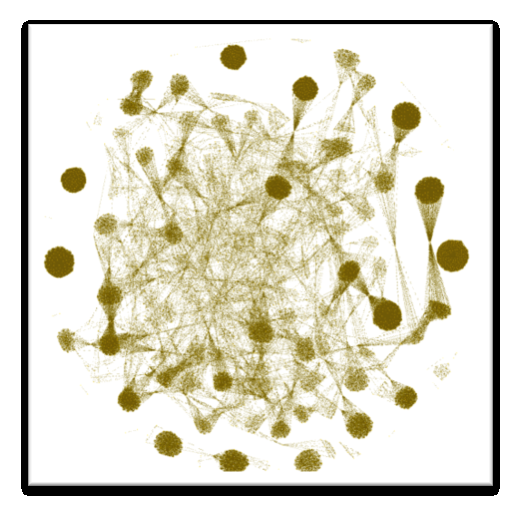
\includegraphics[scale=0.5]{./polish1.eps}
\caption{研磨後のグラフ\label{fig:polish1}}
\end{center}
\end{minipage}

\end{tabular} 
\end{center}
\end{figure} 

研磨のアルゴリズムをAlgorithm \ref{algo:polish}に示す。
ここに示されたアルゴリズムは、非常に効率の悪い方法ではあるが、理解のし易さを優先させている。
実際に内部で実装されているアルゴリズムについては参考文献\cite{Uno2014}に詳しい。
研磨の方法は至ってシンプルで、全ての頂点ペアについて、その類似度(後述)がユーザの指定した閾値以上であれば接続し、
そうでなければ接続しないというルールに従って、新たなグラフを再構成する。


\begin{algorithm}
\caption{グラフ研磨アルゴリズム\label{algo:polish}}
\begin{small}
\begin{algorithmic}[1]
\Function{Polishing}{$G=(V,E),\sigma$}
	\State $V:頂点集合, E:辺集合, \sigma: 類似度下限値$
	\State $E'=\phi$; $V'=\phi$ \Comment 研磨後の辺集合と頂点集合の初期化
	\ForAll{$u\in V$}
		\ForAll{$v\in V$} \Comment \# 全頂点ペア$u,v$について調べる
			\If{$sim(u,v)\ge\sigma$} \Comment 頂点ペア$u,v$が似ていればには新たに辺として加え、似てなければ加えない
				\State $E'=E'\cup (u,v)$
				\State $V'=V'\cup u$
				\State $V'=V'\cup v$
			\EndIf
		\EndFor
	\EndFor
	\State {\bf return}{$(V',E')$}
\EndFunction
\end{algorithmic}
\end{small}
\end{algorithm}

そして新たに構成されたグラフを入力として同様の研磨手法を繰り返し適用し、
グラフの構成に変化がなくなるか、もしくはユーザの指定した最大繰り返し回数に達すれば終了する。
最終的に得られたグラフが研磨グラフである。

次に2つの頂点間の類似度(Algorithm \ref{algo:polish}の6行目:$sim(u,v)$)の定義を示す。
基本的な考え方は「共通の友達が多い友達は友達と考えよう」というものである。
頂点$u,v$に隣接する頂点が図\ref{fig:sim}に示されるような構造を持っていたとしよう。
$u$と$v$に直接の接続はないが、いずれかの頂点に接続された5つの頂点のうち、
頂点3,4の2つの頂点が共通して接続されている。
この情報を利用して類似度は定義される。

\begin{figure}[htbp]
\begin{center}

\begin{minipage}{0.3\hsize}
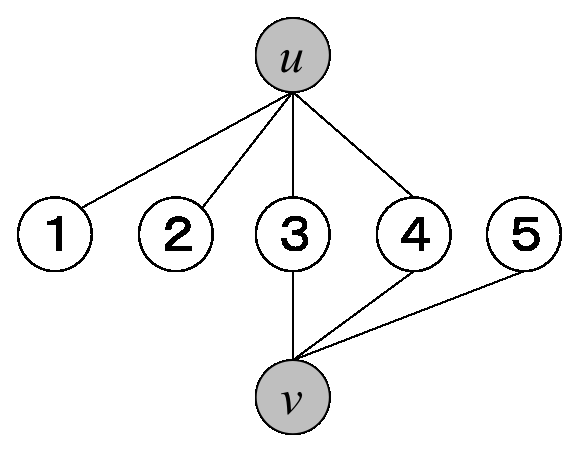
\includegraphics[scale=0.5]{./sim.eps}
\caption{頂点$u,v$の接続関係\label{fig:sim}}
\end{minipage}
\end{center}
\end{figure}

本コマンドでは、表\ref{tbl:simdef}に示されるように、6つの類似度を利用することができる。
類似度の選択は表中に示された\verb|sim=|パラメータを設定することによって行い、
\verb|th=|パラメータによって類似度の下限値を与える。

\begin{table}[htbp]
\begin{center}
\caption{グラフ$G=(V,E)$における節点$u,v$の類似度の定義\label{tbl:simdef}}
%{\small
\begin{tabular}{cllcc}
\hline
\# & 類似度&定義式&sim=パラメータ値&範囲 \\
\hline
1&recemblance    & $\frac{|N(u) \cap N(v)|}{|N(u) \cup N(v)|}$ & R & 0.0〜1.0\\
2&normalized PMI & $\log{\frac{P(u,v)}{P(u)P(v)}}/(-\log{P(u,v)})$ & P  & -1.0〜1.0\\
 &               & $=\frac{|V||N(u) \cap N(v)|}{|N(u)||N(v)|}/(-\log{\frac{|N(u) \cap N(v)|}{|V|}})$ & \\
3&intersection   & $|N(u) \cap N(v)|$ & T & 0〜\\
4&cosine         & $\frac{|N(u) \cap N(v)|}{\sqrt{|N(u)|}\sqrt{|N(v)|}}$ & C  & 0.0〜1.0\\
5&max-confidence & $\frac{|N(u) \cap N(v)|}{\max{(|N(u)|,|N(v)|)}}$ & S  & 0.0〜1.0\\
6&min-confidence & $\frac{|N(u) \cap N(v)|}{\min{(|N(u)|,|N(v)|)}}$ & s  & 0.0〜1.0\\
\hline
\end{tabular} 
\\
{\scriptsize
$N(u)$は頂点$u$に隣接する頂点集合を表す。
$P(u)$は頂点$u$に枝が張られる確率を表し、$P(u)=N(u)/|V|$である。
}
\end{center}
\end{table}

\subsection{例}
本コマンドの入力データである一般グラフは、表\ref{tbl:input}に示されるような、
枝データを節点ペアとして表したCSV形式で与える。
グラフは無向グラフとして扱われ、島が複数あってもよい。
枝を一つも持たない節点は、研磨の対象とならない(友達がいない)ために、節点データを別途入力することはない。
表\ref{tbl:input}のデータを視覚化したグラフを図\ref{fig:inputg}に示す。
以下では、このデータを使いデータ研磨の例を示していく。

\begin{table}[htbp]
\begin{center}
\caption{入力データ(枝データ)\label{tbl:input}}
\begin{tabular}{cc}
\hline
node1&node2 \\
\hline
a&b\\
a&c\\
a&e\\
b&c\\
b&e\\
b&g\\
c&d\\
c&g\\
d&e\\
e&f\\
\hline
\end{tabular} 
\end{center}
\end{table} 

簡単のために、類似度の定義をintersectionとしその下限値を2に設定したとしよう。
すなわち、隣接する節点で共通の節点数(共通する友達の数)が2以上である時に枝を張り、
そうでなければ枝を張らない。
例えば、図\ref{fig:ad}は、図\ref{fig:inputg}から節点$a,b$と連結のある節点を抜き出した部分グラフである。
2つの節点$e,c$を共通に持つため、研磨グラフにおいて、節点$a,b$に枝が張られる。
一方で節点$e,g$(図\ref{fig:eg})は、共通節点は節点$b$だけなので、研磨グラフにおいても枝は張られない。

\begin{figure}[htbp]
\begin{center}
\begin{tabular}{ccc}

\begin{minipage}{0.3\hsize}
\begin{center}
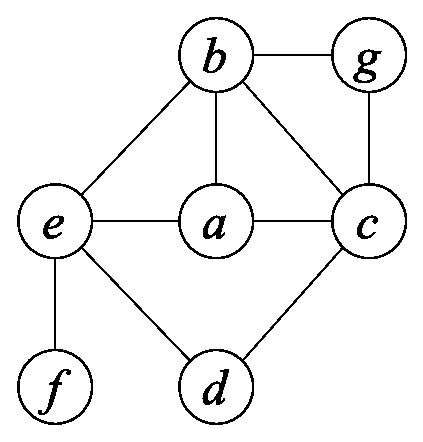
\includegraphics[scale=0.5]{./inputg.eps}
\caption{表\ref{tbl:input}のグラフデータを視覚化\label{fig:inputg}}
\end{center}
\end{minipage}

\begin{minipage}{0.2\hsize}
\begin{center}
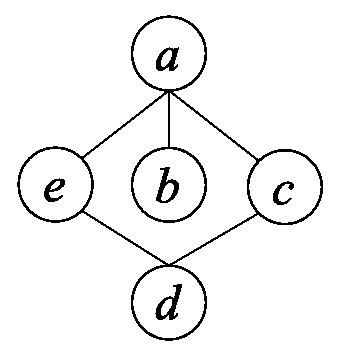
\includegraphics[scale=0.5]{./ad.eps}
\caption{節点$a$と節点$d$の関係\label{fig:ad}}
\end{center}
\end{minipage}

\begin{minipage}{0.2\hsize}
\begin{center}
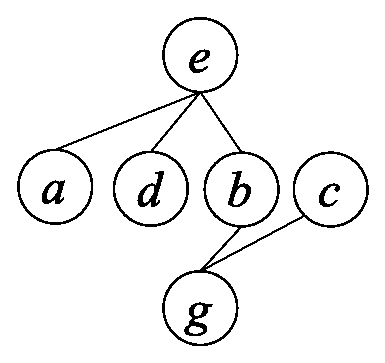
\includegraphics[scale=0.5]{./eg.eps}
\caption{節点$e$と節点$g$の関係\label{fig:eg}}
\end{center}
\end{minipage}

\end{tabular}
\end{center}
\end{figure}

図\ref{fig:ab2}は、節点$a,b$に関連する部分グラフである。
これまでの2つの例と異なる点は、節点$a,b$に直接の接続があることである。
このような場合、2つの考え方を取ることができる。
ひとつは、図\ref{fig:ab1}のように、直接の関係は考慮せず、あくまでも共通の友達関係だけを考慮する方法である。
もう一つの方法は、節点$a,b$をお互いに共通の友達と考え、架空の節点$a',b'$を追加し、$a,b$双方からの接続を仮定する。
よって、直接の接続がある場合、それだけで2人の友達を共通に持つと考える。

\begin{figure}[htbp]
\begin{center}
\begin{tabular}{ccc}

\begin{minipage}{0.3\hsize}
\begin{center}
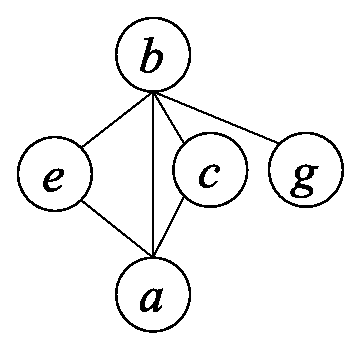
\includegraphics[scale=0.5]{./ab2.eps}
\caption{節点$a$と節点$b$の関係\label{fig:ab2}}
\end{center}
\end{minipage}

\begin{minipage}{0.3\hsize}
\begin{center}
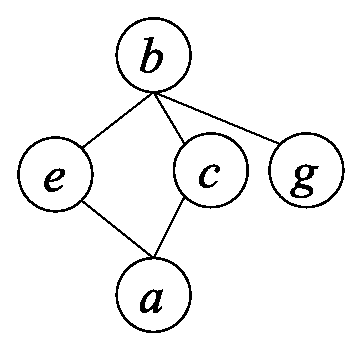
\includegraphics[scale=0.5]{./ab1.eps}
\caption{直接の接続を考慮しない例\label{fig:ab1}}
\end{center}
\end{minipage}

\begin{minipage}{0.3\hsize}
\begin{center}
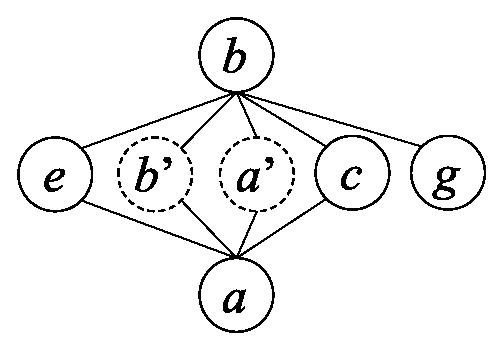
\includegraphics[scale=0.5]{./ab3.eps}
\caption{直接の接続を考慮する例\label{fig:ab3}}
\end{center}
\end{minipage}

\end{tabular}
\end{center}
\end{figure}

以上のようにすべての節点ペアについて新たな接続関係を更新すると、
直接の関係を考慮しない場合は図\ref{fig:polished0}のような研磨グラフが得られ、
直接の関係を考慮する場合は図\ref{fig:polished2}のような研磨グラフが得られる。
そして、新たに得られたこれらの研磨グラフに繰り返しデータ研磨を付していくと、
3回でグラフ構造は変化しなくなり(収束し)、
図\ref{fig:polished1}と図\ref{fig:polished3}が得られる。
直接接続を考慮しない場合は、接続関係がすべて無くなる。
一方で直接接続を考慮する場合は、6つの節点$a,b,c,d,e,g$が互いに接続され、
極大クリークが形成される。
また節点$f$は$e$とのみ接続が残り、これも極大クリーク$e,f$を形成している。
なお、データ研磨を繰り返し適用すると、グラフ構造は安定してくるが、
収束しないケースもあることに注意する。

\begin{figure}[htbp]
\begin{center}
\begin{tabular}{cccc}

\begin{minipage}{0.25\hsize}
\begin{center}
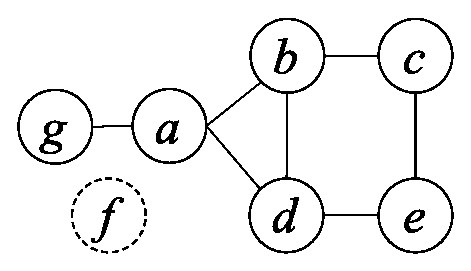
\includegraphics[scale=0.5]{./polished0.eps}
\caption{直接考慮しない1回研磨グラフ\label{fig:polished0}}
\end{center}
\end{minipage}

\begin{minipage}{0.25\hsize}
\begin{center}
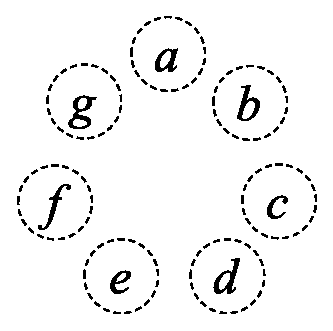
\includegraphics[scale=0.5]{./polished1.eps}
\caption{直接考慮しない3回研磨グラフ\label{fig:polished1}}
\end{center}
\end{minipage}

\begin{minipage}{0.25\hsize}
\begin{center}
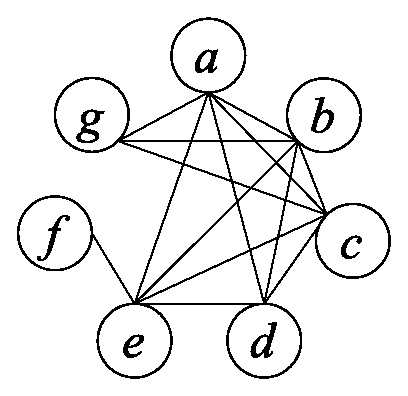
\includegraphics[scale=0.5]{./polished2.eps}
\caption{直接考慮した1回研磨グラフ\label{fig:polished2}}
\end{center}
\end{minipage}

\begin{minipage}{0.25\hsize}
\begin{center}
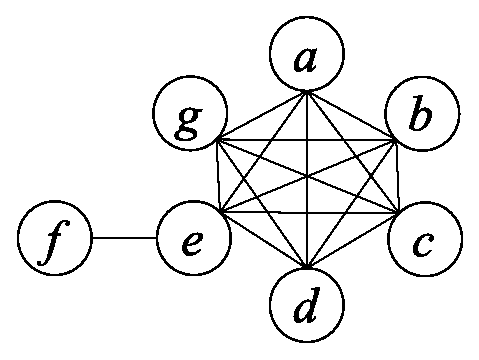
\includegraphics[scale=0.5]{./polished3.eps}
\caption{直接考慮した3回研磨グラフ\label{fig:polished3}}
\end{center}
\end{minipage}

\end{tabular}
\end{center}
\end{figure}

以上は理解のし易さのために、共通する枝の数を類似度と定義してデータ研磨を行ったが、
グラフのサイズが大きくなると、思ったような研磨ができないことが多い。
隣接節点の数が増えるに伴って巨大な次数の頂点が発生し、関係が薄いにも
関わらず十分な数の共通接点を持つ節点ペアにも枝が張られてしまうからである。
%隣接節点の数が増えるに伴って、
%共通節点の数が相対的に低い(関係の薄い)節点ペアが出てくるが、
%共通節点数の下限値が固定されているため、そのような関係の薄い節点ペアにも枝が張られてしまうからである。
そこで、通常は、resemblanceを始めとした、相対的な共通性を評価できる類似度を使う。
類似度としてresenmblanceを用い、その下限値を0.4,0.5として収束するまで研磨したグラフを
図\ref{fig:resemblance04},\ref{fig:resemblance05}にそれぞれ示している。
また図\ref{fig:pmi02}は、類似度としてnormalized PMIを、下限値を0.2とした結果である。

\begin{figure}[htbp]
\begin{center}
\begin{tabular}{ccc}

\begin{minipage}{0.3\hsize}
\begin{center}
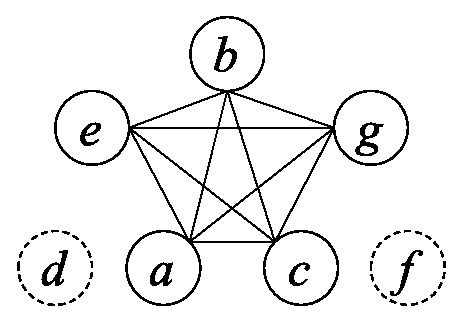
\includegraphics[scale=0.5]{./resemblance04.eps}
\caption{recemblance=0.4による研磨グラフ\label{fig:resemblance04}}
\end{center}
\end{minipage}

\begin{minipage}{0.3\hsize}
\begin{center}
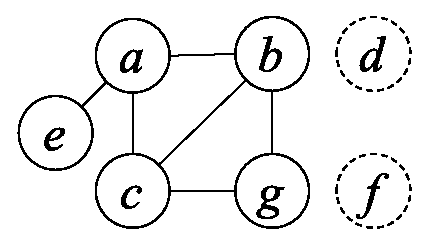
\includegraphics[scale=0.5]{./resemblance05.eps}
\caption{recemblance=0.5による研磨グラフ\label{fig:resemblance05}}
\end{center}
\end{minipage}

\begin{minipage}{0.3\hsize}
\begin{center}
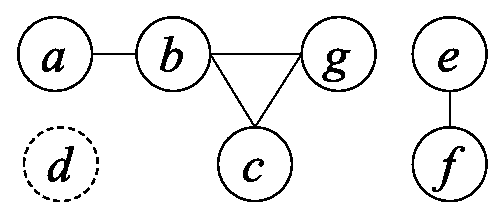
\includegraphics[scale=0.5]{./pmi02.eps}
\caption{normalized PIM=0.2による研磨グラフ\label{fig:pmi02}}
\end{center}
\end{minipage}

\end{tabular}
\end{center}
\end{figure}

なお、出力としては研磨グラフ以外にも表\ref{tbl:stat}に示されるような各種統計を出力することができる(\verb|log=|で指定したファイル)。

\begin{table}[htbp]
\begin{center}
\caption{ログに出力される各種統計\label{tbl:stat}}
%{\small
\begin{tabular}{ll}
\hline
key & 内容 \\
\hline
iter & データ研磨を適用した回数 \\
time & 実行時間\\
nSize0 & データ研磨前のグラフの節点数 \\
eSize0 & データ研磨前のグラフの枝数 \\
dens0  & データ研磨前の枝密度 \\
nSize\# & \#回目のデータ研磨後の節点数 \\
eSize\# & \#回目のデータ研磨後の枝数 \\
dens\#  & \#回目のデータ研磨後の枝密度 \\

\hline
\end{tabular} 
\end{center}
\end{table}


以下にデータ研磨の特徴をまとめておく。
\begin{itemize}
\item 共通する隣接節点の情報にしたがって枝を張り直す。
\item 6つの類似度を選ぶことができ、利用する類似度によって結果は異なってくる。
\item データ研磨を繰り返すことでグラフ構造は安定してくる(多くの場合は収束する)。
\item オリジナルのグラフに比べ極大クリークの数が劇的に少なくなる。
\item 類似度の下限値を低くすると、より大きな極大クリークが形成される。
\end{itemize}


\subsection{書式}
\begin{verbatim}
mpolishing.rb ei= ef= [ni=] [nf=] eo= [no=] [sim=R|P|C|s|S|T] th= [sup=] [-indirect] [iter=] [log=] [T=] [--help]

  ファイル名指定
  ei=    : 枝データファイル
  ef=    : 枝データ上の2つの節点項目名(省略時は"node1,node2")
  ni=    : 節点データファイル
  nf=    : 節点データ上の節点項目名(省略時は"node")
  eo=    : データ研磨後の枝データファイル
  no=    : データ研磨後の節点データファイル
  sim=   : 節点a,bと接続された枝集合を、それぞれA,Bとすると、節点a,bに枝を張るために用いる類似度。
           省略時はRが設定される。
             i: inclusion
             I: both-inclusion
             S: |A∩B|/max(|A|,|B|)
             s: |A∩B|/min(|A|,|B|)
             T (intersection): find pairs having common [threshld] items
             R (resemblance): find pairs s.t. |A\capB|/|A\cupB| >= [threshld]
             P (PMI): find pairs s.t. log (|A\capB|*|all| / (|A|*|B|)) >= [threshld]
             C (cosine distance): find pairs s.t. inner product of their normalized vectors >= [threshld]
  th=    : sim=で指定された類似度について、ここで指定された値以上の節点間に枝を張る。
  sup=   : 類似度計算において、|A∩B|>=supの条件を加える。省略すればsup=0。
  -indirect: 上記類似度計算における隣接節点集合から直接の関係を除外する。
             すなわち、A=A-b, B=B-a として類似度を計算する。
  iter=  : データ研磨の最大繰り返し数(デフォルト=30)
  log=   : パラメータの設定値や収束回数等をkey-value形式のCSVで保存するファイル名
  O=     : データ研磨過程のグラフを保存するディレクトリ名

  その他
  T= : ワークディレクトリ(default:/tmp)
  --help : ヘルプの表示
\end{verbatim}

\subsection{利用例}
\subsubsection*{Example 1: Basic Example}

Use resemblance(sim=R) as similarity measure, the polished graph is obtained by extending the branch at th=0.4.
The number of polishing iterations are converged 3 times as shown in \verb|log1.csv| (iter,4)。
The output result is shown in Figure \ref{fig:resemblance04}.


\begin{Verbatim}[baselinestretch=0.7,frame=single]
$ more dat1.csv
node1,node2
a,b
a,c
a,e
b,c
b,e
b,g
c,d
c,g
d,e
e,f
$ mpolishing.rb i=dat1.csv f=node1,node2 sim=R th=0.4 o=result1.csv log=log1.csv
#MSG# converting graph files into a pair of numbered nodes ...
input-file /tmp/__MTEMP_20042_70166767738540_2, output-file /tmp/__MTEMP_20042_70166767738
540_3
degree threshold: 
first & second scan end: /tmp/__MTEMP_20042_70166767738540_2
file read end: /tmp/__MTEMP_20042_70166767738540_2
iterative scan: #nodes=7, #edges = 20
forwardstar graph: /tmp/__MTEMP_20042_70166767738540_2 ,#nodes 7(7,7) ,#edges 20
#MSG# polishing iteration #0 (tra size=61
sspc_20140215 R -l 0 /tmp/__MTEMP_20042_70166767738540_3 0.4 /tmp/__MTEMP_20042_7016676773
8540_2
trsact: /tmp/__MTEMP_20042_70166767738540_3 ,#transactions 7 ,#items 7 ,size 27 extracted 
database: #transactions 7 ,#items 7 ,size 27
 output to: /tmp/__MTEMP_20042_70166767738540_2
separated at 0
11 pairs are found
0,1,2,4, :1.000000  (0)
0,1,2,4,6, :1.000000  (0)
0,1,2,3,6, :1.000000  (0)
2,3,4, :1.000000  (0)
0,1,3,4,5, :1.000000  (0)
4,5, :1.000000  (0)
1,2,6, :1.000000  (0)
come
input-file /tmp/__MTEMP_20042_70166767738540_2, output-file /tmp/__MTEMP_20042_70166767738
540_3
degree threshold: 
first & second scan end: /tmp/__MTEMP_20042_70166767738540_2
file read end: /tmp/__MTEMP_20042_70166767738540_2
iterative scan: #nodes=7, #edges = 22
forwardstar graph: /tmp/__MTEMP_20042_70166767738540_2 ,#nodes 7(7,7) ,#edges 22
#MSG# polishing iteration #1 (tra size=65
sspc_20140215 R -l 0 /tmp/__MTEMP_20042_70166767738540_3 0.4 /tmp/__MTEMP_20042_7016676773
8540_2
trsact: /tmp/__MTEMP_20042_70166767738540_3 ,#transactions 7 ,#items 7 ,size 29 extracted 
database: #transactions 7 ,#items 7 ,size 29
 output to: /tmp/__MTEMP_20042_70166767738540_2
separated at 0
11 pairs are found
0,1,2,3,4,6, :1.000000  (0)
0,1,2,4,6, :1.000000  (0)
0,1,2,4,6, :1.000000  (0)
0,3, :1.000000  (0)
0,1,2,4,5, :1.000000  (0)
4,5, :1.000000  (0)
0,1,2,6, :1.000000  (0)
come
input-file /tmp/__MTEMP_20042_70166767738540_2, output-file /tmp/__MTEMP_20042_70166767738
540_3
degree threshold: 
first & second scan end: /tmp/__MTEMP_20042_70166767738540_2
file read end: /tmp/__MTEMP_20042_70166767738540_2
iterative scan: #nodes=6, #edges = 22
forwardstar graph: /tmp/__MTEMP_20042_70166767738540_2 ,#nodes 7(7,7) ,#edges 22
#MSG# polishing iteration #2 (tra size=63
sspc_20140215 R -l 0 /tmp/__MTEMP_20042_70166767738540_3 0.4 /tmp/__MTEMP_20042_7016676773
8540_2
trsact: /tmp/__MTEMP_20042_70166767738540_3 ,#transactions 7 ,#items 7 ,size 28 extracted 
database: #transactions 7 ,#items 7 ,size 28
 output to: /tmp/__MTEMP_20042_70166767738540_2
separated at 0
10 pairs are found
0,1,2,4,6, :1.000000  (0)
0,1,2,4,6, :1.000000  (0)
0,1,2,4,6, :1.000000  (0)
 :1.000000  (0)
0,1,2,4,5,6, :1.000000  (0)
4,5, :1.000000  (0)
0,1,2,4,6, :1.000000  (0)
come
input-file /tmp/__MTEMP_20042_70166767738540_2, output-file /tmp/__MTEMP_20042_70166767738
540_3
degree threshold: 
first & second scan end: /tmp/__MTEMP_20042_70166767738540_2
file read end: /tmp/__MTEMP_20042_70166767738540_2
iterative scan: #nodes=5, #edges = 20
forwardstar graph: /tmp/__MTEMP_20042_70166767738540_2 ,#nodes 7(7,7) ,#edges 20
#MSG# polishing iteration #3 (tra size=57
sspc_20140215 R -l 0 /tmp/__MTEMP_20042_70166767738540_3 0.4 /tmp/__MTEMP_20042_7016676773
8540_2
trsact: /tmp/__MTEMP_20042_70166767738540_3 ,#transactions 7 ,#items 7 ,size 25 extracted 
database: #transactions 7 ,#items 7 ,size 25
 output to: /tmp/__MTEMP_20042_70166767738540_2
separated at 0
10 pairs are found
0,1,2,4,6, :1.000000  (0)
0,1,2,4,6, :1.000000  (0)
0,1,2,4,6, :1.000000  (0)
 :1.000000  (0)
0,1,2,4,6, :1.000000  (0)
 :1.000000  (0)
0,1,2,4,6, :1.000000  (0)
come
input-file /tmp/__MTEMP_20042_70166767738540_2, output-file /tmp/__MTEMP_20042_70166767738
540_3
degree threshold: 
first & second scan end: /tmp/__MTEMP_20042_70166767738540_2
file read end: /tmp/__MTEMP_20042_70166767738540_2
iterative scan: #nodes=5, #edges = 20
forwardstar graph: /tmp/__MTEMP_20042_70166767738540_2 ,#nodes 7(7,7) ,#edges 20
#MSG# converting the numbered nodes into original name ...
#END# /Users/stephane/.rvm/rubies/ruby-1.9.3-p448/bin/mpolishing.rb i=dat1.csv f=node1,nod
e2 sim=R th=0.4 o=result1.csv log=log1.csv
$ more result1.csv
node1,node2
a,b
a,c
a,e
a,g
b,c
b,e
b,g
c,e
c,g
e,g
$ more log1.csv
key,value
i=,dat1.csv
f=,"node1,node2"
sim=,R
th=,0.4
o=,result1.csv
log=,log1.csv
-int,false
-indirect,false
iter,4
time,0.113653
nSize0,7
eSize0,10
dens0,0.4761904762
nSize1,7
eSize1,11
dens1,0.5238095238
nSize2,6
eSize2,11
dens2,0.7333333333
nSize3,5
eSize3,10
dens3,1
nSize4,5
eSize4,10
dens4,1
\end{Verbatim}
\subsubsection*{Example 2: Polishing by PMI}

Use normalized PMI(sim=P) as similarity measure, the polished graph is obtained by extending the branch at th=0.2.
The output result is shown in Figure \ref{fig:pmi02}.



\begin{Verbatim}[baselinestretch=0.7,frame=single]
$ mpolishing.rb i=dat1.csv f=node1,node2 sim=P th=0.2 o=result2.csv
#MSG# converting graph files into a pair of numbered nodes ...
input-file /tmp/__MTEMP_20101_70350905868560_2, output-file /tmp/__MTEMP_20101_70350905868
560_3
degree threshold: 
first & second scan end: /tmp/__MTEMP_20101_70350905868560_2
file read end: /tmp/__MTEMP_20101_70350905868560_2
iterative scan: #nodes=7, #edges = 20
forwardstar graph: /tmp/__MTEMP_20101_70350905868560_2 ,#nodes 7(7,7) ,#edges 20
#MSG# polishing iteration #0 (tra size=61
sspc_20140215 P -l 0 /tmp/__MTEMP_20101_70350905868560_3 0.2 /tmp/__MTEMP_20101_7035090586
8560_2
trsact: /tmp/__MTEMP_20101_70350905868560_3 ,#transactions 7 ,#items 7 ,size 27 extracted 
database: #transactions 7 ,#items 7 ,size 27
 output to: /tmp/__MTEMP_20101_70350905868560_2
separated at 0
5 pairs are found
0,1,2,4, :1.000000  (0)
0,1,2,4,6, :1.000000  (0)
0,1,2,3,6, :1.000000  (0)
2,3,4, :1.000000  (0)
0,1,3,4,5, :1.000000  (0)
4,5, :1.000000  (0)
1,2,6, :1.000000  (0)
come
input-file /tmp/__MTEMP_20101_70350905868560_2, output-file /tmp/__MTEMP_20101_70350905868
560_3
degree threshold: 
first & second scan end: /tmp/__MTEMP_20101_70350905868560_2
file read end: /tmp/__MTEMP_20101_70350905868560_2
iterative scan: #nodes=6, #edges = 10
forwardstar graph: /tmp/__MTEMP_20101_70350905868560_2 ,#nodes 7(7,7) ,#edges 10
#MSG# polishing iteration #1 (tra size=39
sspc_20140215 P -l 0 /tmp/__MTEMP_20101_70350905868560_3 0.2 /tmp/__MTEMP_20101_7035090586
8560_2
trsact: /tmp/__MTEMP_20101_70350905868560_3 ,#transactions 7 ,#items 7 ,size 16 extracted 
database: #transactions 7 ,#items 7 ,size 16
 output to: /tmp/__MTEMP_20101_70350905868560_2
separated at 0
5 pairs are found
0,1, :1.000000  (0)
0,1,2,6, :1.000000  (0)
1,2,6, :1.000000  (0)
 :1.000000  (0)
4,5, :1.000000  (0)
4,5, :1.000000  (0)
1,2,6, :1.000000  (0)
come
input-file /tmp/__MTEMP_20101_70350905868560_2, output-file /tmp/__MTEMP_20101_70350905868
560_3
degree threshold: 
first & second scan end: /tmp/__MTEMP_20101_70350905868560_2
file read end: /tmp/__MTEMP_20101_70350905868560_2
iterative scan: #nodes=6, #edges = 10
forwardstar graph: /tmp/__MTEMP_20101_70350905868560_2 ,#nodes 7(7,7) ,#edges 10
#MSG# converting the numbered nodes into original name ...
#END# /Users/stephane/.rvm/rubies/ruby-1.9.3-p448/bin/mpolishing.rb i=dat1.csv f=node1,nod
e2 sim=P th=0.2 o=result2.csv
$ more result2.csv
node1,node2
a,b
b,c
b,g
c,g
e,f
\end{Verbatim}
\subsubsection*{Example 3: Polish once at intersection}

Based on the explanation in the previous example. Use intersection(sim=T) as similarity measure, consider cases with 2 or more (th=2) branch extension with direct connection. Polish graph with 1 iteration (iter=1).
The output result is shown in Figure \ref{fig:polished2}.



\begin{Verbatim}[baselinestretch=0.7,frame=single]
$ mpolishing.rb i=dat1.csv f=node1,node2 sim=T th=2 iter=1 o=result3.csv
#MSG# converting graph files into a pair of numbered nodes ...
input-file /tmp/__MTEMP_20151_70168512314200_2, output-file /tmp/__MTEMP_20151_70168512314
200_3
degree threshold: 
first & second scan end: /tmp/__MTEMP_20151_70168512314200_2
file read end: /tmp/__MTEMP_20151_70168512314200_2
iterative scan: #nodes=7, #edges = 20
forwardstar graph: /tmp/__MTEMP_20151_70168512314200_2 ,#nodes 7(7,7) ,#edges 20
#MSG# polishing iteration #0 (tra size=61
sspc_20140215 T -l 0 /tmp/__MTEMP_20151_70168512314200_3 2.0 /tmp/__MTEMP_20151_7016851231
4200_2
trsact: /tmp/__MTEMP_20151_70168512314200_3 ,#transactions 7 ,#items 7 ,size 27 extracted 
database: #transactions 7 ,#items 7 ,size 27
 output to: /tmp/__MTEMP_20151_70168512314200_2
separated at 0
14 pairs are found
0,1,2,4, :1.000000  (0)
0,1,2,4,6, :1.000000  (0)
0,1,2,3,6, :1.000000  (0)
2,3,4, :1.000000  (0)
0,1,3,4,5, :1.000000  (0)
4,5, :1.000000  (0)
1,2,6, :1.000000  (0)
come
input-file /tmp/__MTEMP_20151_70168512314200_2, output-file /tmp/__MTEMP_20151_70168512314
200_3
degree threshold: 
first & second scan end: /tmp/__MTEMP_20151_70168512314200_2
file read end: /tmp/__MTEMP_20151_70168512314200_2
iterative scan: #nodes=7, #edges = 28
forwardstar graph: /tmp/__MTEMP_20151_70168512314200_2 ,#nodes 7(7,7) ,#edges 28
#MSG# converting the numbered nodes into original name ...
#END# /Users/stephane/.rvm/rubies/ruby-1.9.3-p448/bin/mpolishing.rb i=dat1.csv f=node1,nod
e2 sim=T th=2 iter=1 o=result3.csv
$ more result3.csv
node1,node2
a,b
a,c
a,d
a,e
a,g
b,c
b,d
b,e
b,g
c,d
c,e
c,g
d,e
e,f
\end{Verbatim}
\subsubsection*{Example 4: Exclude direct connection}

When \verb|-indirect| is specified, direct connection is ignored when calculating degree of similarity.
The output graph is shown in Figure \ref{fig:polished1}, to remove all branches, branch data is not returned after polishing.


\begin{Verbatim}[baselinestretch=0.7,frame=single]
$ mpolishing.rb i=dat1.csv f=node1,node2 sim=T th=2 o=result4.csv -indirect
#MSG# converting graph files into a pair of numbered nodes ...
input-file /tmp/__MTEMP_20194_70296082596580_2, output-file /tmp/__MTEMP_20194_70296082596
580_3
degree threshold: 
first & second scan end: /tmp/__MTEMP_20194_70296082596580_2
file read end: /tmp/__MTEMP_20194_70296082596580_2
iterative scan: #nodes=7, #edges = 20
forwardstar graph: /tmp/__MTEMP_20194_70296082596580_2 ,#nodes 7(7,7) ,#edges 20
#MSG# polishing iteration #0 (tra size=47
sspc_20140215 T -l 0 /tmp/__MTEMP_20194_70296082596580_3 2.0 /tmp/__MTEMP_20194_7029608259
6580_2
trsact: /tmp/__MTEMP_20194_70296082596580_3 ,#transactions 7 ,#items 7 ,size 20 extracted 
database: #transactions 7 ,#items 7 ,size 20
 output to: /tmp/__MTEMP_20194_70296082596580_2
separated at 0
6 pairs are found
1,2,4, :1.000000  (0)
0,2,4,6, :1.000000  (0)
0,1,3,6, :1.000000  (0)
2,4, :1.000000  (0)
0,1,3,5, :1.000000  (0)
4, :1.000000  (0)
1,2, :1.000000  (0)
come
input-file /tmp/__MTEMP_20194_70296082596580_2, output-file /tmp/__MTEMP_20194_70296082596
580_3
degree threshold: 
first & second scan end: /tmp/__MTEMP_20194_70296082596580_2
file read end: /tmp/__MTEMP_20194_70296082596580_2
iterative scan: #nodes=6, #edges = 12
forwardstar graph: /tmp/__MTEMP_20194_70296082596580_2 ,#nodes 7(7,7) ,#edges 12
#MSG# polishing iteration #1 (tra size=31
sspc_20140215 T -l 0 /tmp/__MTEMP_20194_70296082596580_3 2.0 /tmp/__MTEMP_20194_7029608259
6580_2
trsact: /tmp/__MTEMP_20194_70296082596580_3 ,#transactions 7 ,#items 7 ,size 12 extracted 
database: #transactions 7 ,#items 7 ,size 12
 output to: /tmp/__MTEMP_20194_70296082596580_2
separated at 0
0 pairs are found
1,3,6, :1.000000  (0)
0,2,3, :1.000000  (0)
1,4, :1.000000  (0)
0,1, :1.000000  (0)
2, :1.000000  (0)
 :1.000000  (0)
0, :1.000000  (0)
come
input-file /tmp/__MTEMP_20194_70296082596580_2, output-file /tmp/__MTEMP_20194_70296082596
580_3
degree threshold: 
first & second scan end: /tmp/__MTEMP_20194_70296082596580_2
file read end: /tmp/__MTEMP_20194_70296082596580_2
iterative scan: #nodes=0, #edges = 0
forwardstar graph: /tmp/__MTEMP_20194_70296082596580_2 ,#nodes 0(0,0) ,#edges 0
#MSG# polishing iteration #2 (tra size=6
sspc_20140215 T -l 0 /tmp/__MTEMP_20194_70296082596580_3 2.0 /tmp/__MTEMP_20194_7029608259
6580_2
trsact: /tmp/__MTEMP_20194_70296082596580_3 ,#transactions 2 ,#items 4 ,size 1 extracted d
atabase: #transactions 2 ,#items 4 ,size 1
 output to: /tmp/__MTEMP_20194_70296082596580_2
separated at 0
0 pairs are found
 :1.000000  (0)
3, :1.000000  (0)
come
input-file /tmp/__MTEMP_20194_70296082596580_2, output-file /tmp/__MTEMP_20194_70296082596
580_3
degree threshold: 
first & second scan end: /tmp/__MTEMP_20194_70296082596580_2
file read end: /tmp/__MTEMP_20194_70296082596580_2
iterative scan: #nodes=0, #edges = 0
forwardstar graph: /tmp/__MTEMP_20194_70296082596580_2 ,#nodes 0(0,0) ,#edges 0
#MSG# converting the numbered nodes into original name ...
#END# /Users/stephane/.rvm/rubies/ruby-1.9.3-p448/bin/mpolishing.rb i=dat1.csv f=node1,nod
e2 sim=T th=2 o=result4.csv -indirect
$ more result4.csv
node1,node2
\end{Verbatim}





\section{mtra2g.rb - Construct item similarity graph\label{sect:mtra2g}}

This command constructs a general graph (referred to as "similarity graph") to reflect the structural similarity between items within the transaction data . 
The \verb|lcm|  \cite{UnoWeb}  command is used in mtra2g.rb.  
Degree of similarity is defined by the co-occurrence information of two items, by extending an edge between items a similarity measure higher than the lower limit specified by the user.
Probability of item occurrence (support) and number of occurrence can be specified to derive degree of similarity. In addition, resemblance and the normalized PMI can be added as additional criteria. The definition of each is shown in Table \ref{tbl mt2g_simdef}.


\begin{table}[htbp]
\begin{center}
\caption{Definition of degree of similarity between items $a$ and $b$ \label{tbl:mt2g_simdef}}
%{\small
\begin{tabular}{cllcc}
\hline
Degree of similarity&Formula&Parameter&Range \\
\hline
support        & $\frac{|Occ(a,b)|}{n}$ & s= & 0.0〜1.0 \\
occurence      & $|Occ(a,b)|$ & S= & 1〜 \\
recemblance    & $\frac{|Occ(a) \cap Occ(b)|}{|Occ(a) \cup Occ(b)|}$ & sim=R th= & 0.0〜1.0\\
normalized PMI & $\log{\frac{P(a,b)}{P(a)P(b)}}/(-\log{P(a,b)})$ & sim=P th=  & -1.0〜1.0\\
               & $=\frac{n|Occ(a) \cap Occ(b)|}{|Occ(a)||Occ(b)|}/(-\log{\frac{|Occ(a) \cap Occ(b)|}{n}})$ & \\
\hline
\end{tabular} 
\\
{\scriptsize
$n$ represents the total number of transactions. 
$Occ(a)$ represents the transaction set which item a appeared. 
$P(a)$ represents the probability of occurrence for item a denoted as $P(a)=Occ(a)/n$.
}
\end{center}
\end{table}

The same key-based transaction data is used as the input data used in \hyperref[sect:mitemset]{mitemset.rb} command is used as input data in this section as shown in (Table \ref{tbl:mt2g_key}). 
The data is converted from key based to transaction based formatted data by \verb|mtra| command in MCMD package as shown in Table \ref{tbl:mt2g_tra}. 

Given the input data, Table \ref{tbl:mt2g_out1} shows the result of similarity graph with 2 or more  occurrence, the graph structure is shown in Figure \ref{fig:mt2g_out1} . 


\begin{table}[htbp]
\begin{center}
\begin{tabular}{ccc}

\begin{minipage}{0.25\hsize}
\begin{center}
\caption{Key based data\label{tbl:mt2g_key}}
{\small
\begin{tabular}{cc}
\hline
key&item \\
\hline
T1&C \\
T1&E \\
T2&D \\
T2&E \\
T2&F \\
:&: \\ \hline
\end{tabular} 
}
\end{center}
\end{minipage}

\begin{minipage}{0.25\hsize}
\begin{center}
\caption{Tra based data\label{tbl:mt2g_tra}}
{\small
\begin{tabular}{ll}
\hline
id&item \\
\hline
T1&C E \\
T2&D E F \\
T3&A B D F \\
T4&B D F \\
T5&A B D E \\
T6&A B D E F \\
\hline
\end{tabular} 
}
\end{center}
\end{minipage}

\begin{minipage}{0.5\hsize}
\begin{center}
\caption{Item similarity graph with 2 or more occurrence. The probability of occurrence indicates the number of occurrence. When sim= parameter is specified, the value will be shown in the final column (void). 
\label{tbl:mt2g_out1}}
{\small
\begin{tabular}{cccc}
\hline
node1&node2&support&void\\
\hline
a&b&0.6&\\
a&d&0.4&\\
a&f&0.4&\\
d&b&0.6&\\
e&d&0.4&\\
f&b&0.6&\\
f&d&0.6&\\
\hline
\end{tabular} 
}
\end{center}
\end{minipage}


\end{tabular} 
\end{center}
\end{table} 

\begin{figure}[htbp]
\begin{center}
\begin{minipage}{0.3\hsize}
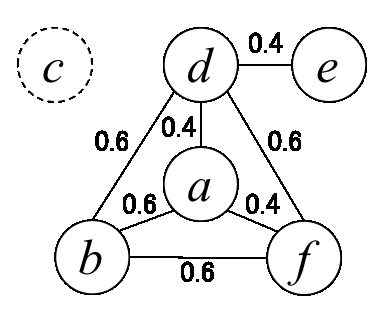
\includegraphics[scale=0.6]{./simg.eps}
\caption{The corresponding similarity graph is shown in Figure \ref{tbl:mt2g_out1}. Each edge shows the co-occurrence probability of the two items. \label{fig:mt2g_out1}}
\end{minipage}
\end{center}
\end{figure}


\subsection{Format}
\begin{verbatim}
Format) mtra2g.rb i= tid= item= [on=] oe= s= [sim=] [th=] [log=] [T=] [--help]

  Specification of file name
  i=     : Transaction data file 
  tid=   : Field name of Transaction ID
  item=  : Field name of item 
  on=    : Output file (node)
  oe=    : Output file (side:node pair)
  s=     : Minimum support [(specified by percentage of total number of transactions): real number between 0 and 1]
  S=     : Minimum support [(specify the number of transactions): integer above 1]
         : When both s=,S= is not specified, default setting becomes S=1. 
  sim=   : Degree of similarity
           R: resemblance
           P: normalized PMI
           When not specified, the edge is extended based on the criteria specified at s= and S=. 
  th=    :  Extend an edge between items with the degree of similarity above  the threshold value specified here. Type of degree of similarity is specified at sim=.
 log=   : Specify file name to save the parameter settings in key-based CSV format. 

  Others
  T= : Working directory (default:/tmp)
  --help : Help information 
\end{verbatim}

\subsection{Examples}
\subsubsection*{例1: 基本例}

出現件数が2件以上の類似度グラフ。
上述の解説の中で示した例。


\begin{Verbatim}[baselinestretch=0.7,frame=single]
$ more dat1.csv
tid,item
T1,C
T1,E
T2,D
T2,E
T2,F
T3,A
T3,B
T3,D
T3,F
T4,B
T4,D
T4,F
T5,A
T5,B
T5,D
T5,E
T6,A
T6,B
T6,D
T6,E
T6,F
$ mtra2g.rb  S=2 tid=tid item=item i=dat1.csv eo=edge1.csv
#MSG# converting a named item into a numbered item ...
#MSG# run lcm enumerating 2 itemset ...
#MSG# creating the edge file ...
#END# /usr/bin/mtra2g.rb S=2 tid=tid item=item i=dat1.csv eo=edge1.csv
$ more edge1.csv
node1,node2,support,void
A,B,0.5,
A,D,0.5,
A,E,0.3333333333,
A,F,0.3333333333,
B,D,0.6666666667,
E,B,0.3333333333,
E,D,0.5,
F,B,0.5,
F,D,0.6666666667,
F,E,0.3333333333,
\end{Verbatim}
\subsubsection*{例2: resemblanceを追加}

例1に加えてresemblanceが0.4以上を類似度条件に加える。
また\verb|no=|を指定することで、節点情報としてアイテム単独の出現頻度を出力する。


\begin{Verbatim}[baselinestretch=0.7,frame=single]
$ mtra2g.rb  S=2 sim=R th=0.4 tid=tid item=item i=dat1.csv eo=edge2.csv no=node2.csv
#MSG# converting a named item into a numbered item ...
#MSG# run lcm enumerating 2 itemset ...
#MSG# creating the edge file ...
#MSG# creating the node file ...
#END# /usr/bin/mtra2g.rb S=2 sim=R th=0.4 tid=tid item=item i=dat1.csv eo=edge2.csv no=nod
e2.csv
$ more node2.csv
node,support
A,0.5
B,0.6666666667
C,0.1666666667
D,0.8333333333
E,0.6666666667
F,0.6666666667
$ more edge2.csv
node1,node2,support,resemblance
A,B,0.5,0.75
A,D,0.5,0.6
A,E,0.3333333333,0.4
A,F,0.3333333333,0.4
B,D,0.6666666667,0.8
E,D,0.5,0.5
F,B,0.5,0.6
F,D,0.6666666667,0.8
\end{Verbatim}





\section{mclique.rb - Enumerate Maximal Cliques\label{sect:mclique}}

This command enumerates the maximal cliques from general graph. The \verb|mace| command \cite{UnoWeb} is used in mclique.rb. 
Given $G=(V,E)$ is an undirected graph with node (referred as vertex) set $V$ and edge set $E$, 
a clique is a subset of its nodes (or vertices)  $V$ such that every two nodes in the subset are connected by an edge in the subgraph of $G$ . 
A maximal clique is a clique that is not an exclusive subset of a larger clique (Figure \ref{fig:clique}).

\begin{figure}[htbp]
\begin{center}
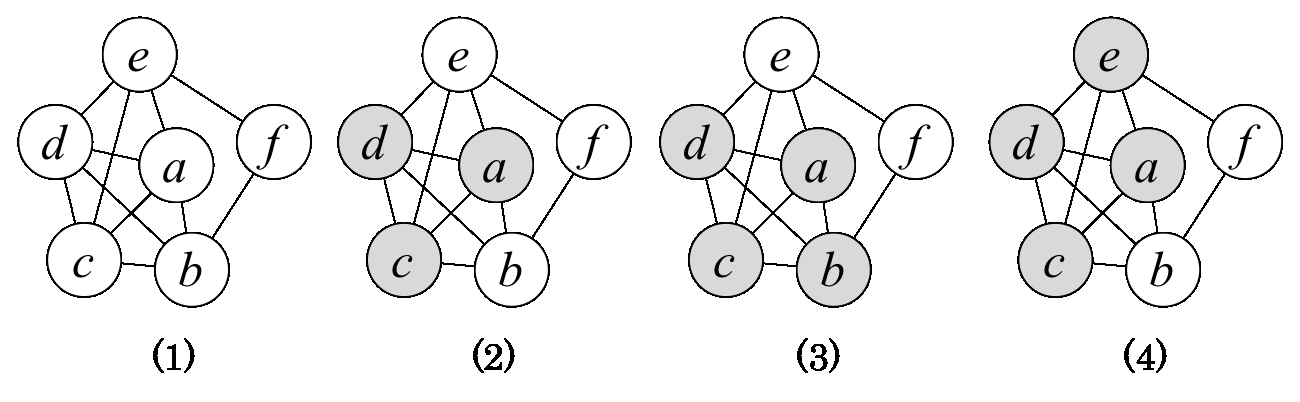
\includegraphics[scale=0.5]{./clique.eps}
\caption{General graph (1) consists of a clique in the subgraph indicated by the shaded nodes in (2),  but the subset is not maximal clique as shown in (3) and (4).  
On the other hand, (3) and (4) are maximal cliques since they are not a subset of other cliques. 
(3) and (4) is constructed by 4 nodes, with 3 common nodes. 
\label{fig:clique}}
\end{center}
\end{figure} 

In general cases, the data points grow to a huge number when enumerating maximal cliques. This is due to the fact that the nodes of maximal cliques overlap each other as shown in Figure \ref{fig:clique} (3) and (4). 
To date, there are  several proposals to overcome this problem. 
One proposal is to treat as a complete graph if the density reaches a particular level, this is known as pseudo clique. However, sometimes more pseudo cliques are enumerated then maximal cliques, and the fundamental problem is not resolved. 
Another approach is to merge similar cliques after enumerating maximal cliques, which make use of different available clustering algorithms. Although this approach is rather promising, the run time required could be a problem depending on the number of maximal cliques enumerated. The third approach is to polish the general graph before enumeration (this cleaning technique is referred to as "data polishing") to reduce the number of maximal cliques enumerated.  
Data polishing is recently proposed by Professor Uno \cite{Uno2014}, if the statistical proof of data polishing becomes more apparent, clique enumeration will become an effective methodology. 
In section  \ref{sect:mpolishing}, this technique is implemented in \verb|mpolishing.rb| command. When mpolishing is used in conjunction with this command, the number of maximal cliques  enumerated can be reduced drastically without altering the nature of the graph. 

Table \ref{tbl:cl_input} shows the input data for this command, edge data is represented in node pair in CSV format (corresponds to Figure \ref{fig:clique} (1)). 
The graph is treated as undirected graph and may have more than one island.  

Given the graph data, maximal cliques are enumerated as shown in Table \ref{tbl:cl_output}. 

The field \verb|id| denotes clique ID, this field identifies records in the same cliques. 
Clique where \verb|id|=2 corresponds to Figure \ref{fig:clique}(4), 
and clique where \verb|id|=3 corresponds to Figure \ref{fig:clique}(3). 
In addition, maximal cliques comprised of the nodes $\{e,f\}$ and $\{b,f\}$ are enumerated. 
The last column \verb|size| contains the number of nodes that made up the maximal cliques. 

%In addition, when parameters \verb|no=,ne=| are specified, the maximal clique of nodes in graph for the clique enumerated can be saved in output.  (node is referred to as clique node, and graph is referred clique node graph). 

%If there is at least 1 common nodes for 2 cliques, an edge is added between the cliques. 
 
% Table \ref{tbl:cl_output} shows the maximal clique based on the clique node graph in Figure \ref{fig:cl_clnodeg}, the output CSV data is shown in Table \ref{tbl:cl_node},\ref{tbl:cl_edge}.

\vspace{1em}

\begin{table}[htbp]
\begin{center}
\begin{tabular}{cc}

\begin{minipage}{0.5\hsize}
\begin{center}
\caption{Input Data (Edge data)\label{tbl:cl_input}}
{\small
\begin{tabular}{cc}
\hline
node1&node2 \\
\hline
a&b \\
a&c \\
a&d \\
a&e \\
b&c \\
b&d \\
b&f \\
c&d \\
c&e \\
d&e \\
e&f \\
\hline
\end{tabular} 
}
\end{center}
\end{minipage}

\begin{minipage}{0.5\hsize}
\begin{center}
\caption{Output Results\label{tbl:cl_output}}
{\small
\begin{tabular}{cccc}
\hline
id&node1&node2&size\\
\hline
0&e&f&2\\
1&b&f&2\\
2&a&c&4\\
2&a&d&4\\
2&a&e&4\\
2&c&d&4\\
2&c&e&4\\
2&d&e&4\\
3&a&b&4\\
3&a&c&4\\
3&a&d&4\\
3&b&c&4\\
3&b&d&4\\
3&c&d&4\\
\hline
\end{tabular} 
}
\end{center}
\end{minipage}

\end{tabular} 
\end{center}
\end{table} 

%\begin{figure}[htbp]
%\begin{center}
%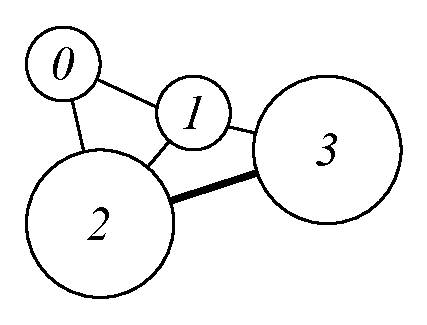
\includegraphics[scale=0.5]{./clnodeg.eps}
%\caption{Clique node graph. Table \ref{tbl:cl_output} shows 4 maximal cliques and its respective nodes for the graph. 
%The number inside the node represents an ID, the saize of the nodes are drawn in proportion to the number of nodes constituting the clique. 
%For example, clique node "2", is made up of 4 nodes $a,c,d,e$, while clique node "0" is made up of 2 nodes $e,f$. 
%When there are more than 1 common nodes between clique, an edge is extended, the thickness of the edge is drawn in proportion to the ratio. 
%For example, there is 1 common node $e$ between clique node "2" and "0".
%There is no edge between clique node "0" and "3" since there is no common node. 
%\label{fig:cl_clnodeg}}
%\end{center}
%\end{figure} 


%\begin{table}[htbp]
%\begin{center}
%\begin{tabular}{cc}

%\begin{minipage}{0.5\hsize}
%\begin{center}
%\caption{Clique node graph in node data\label{tbl:cl_node}}
%{\small
%\begin{tabular}{cc}
%\hline
%node&size \\
%\hline
%0&2 \\
%1&2 \\
%2&4 \\
%3&4 \\
%\hline
%\end{tabular} 
%}
%\end{center}
%\end{minipage}

%\begin{minipage}{0.5\hsize}
%\begin{center}
%\caption{Clique node graph in edge data\label{tbl:cl_edge}}
%{\small
%\begin{tabular}{ccc}
%\hline
%node1&node2&common \\
%\hline
%0&1&1 \\
%0&2&1 \\
%1&3&1 \\
%2&3&3 \\
%\hline
%\end{tabular} 
%}
%\end{center}
%\end{minipage}

%\end{tabular} 
%\end{center}
%\end{table} 



\subsection{Format}
\begin{verbatim}
Format) mclique.rb i= f= [o=] [l=] [u=] [-all] [-node] [-all] [-int] [log=] [T=] [--help] 

  Specify File Name 
  i=     : Edge data file 
  f=     : Column name of 2 nodes in edge data (invalid parameter when -int is specified)
  o=     : Output file (Clique ID-Edge: cliqueID-node can be modified when -node is specified)
  l=     :  Minimal number of nodes constructing the clique (clique smaller than the value 
  specified will not be enumerated) 
 u=     : Maximal number of nodes constructing the clique (clique larger than the value 
 specified will not be enumerated)
  -node  : Output in clique ID-node name pair format 
  -all   : Enumerate all cliques instead of only maximal cliques
  -int   : Process items as integers
  log=   : File name of the parameter settings saved in key based CSV format

 Others
  T= : Working directory (default:/tmp)
  --help : Help information 
\end{verbatim}

\subsection{Examples}
\subsubsection*{Example 1: Basic Example}

Example illustrated from the above section.


\begin{Verbatim}[baselinestretch=0.7,frame=single]
$ more dat1.csv
node1,node2
a,b
a,c
a,d
a,e
b,c
b,d
b,f
c,d
c,e
d,e
e,f
$ mclique.rb i=dat1.csv f=node1,node2 o=result1.csv log=log1.csv
/Users/stephane/.rvm/gems/ruby-1.9.3-p448/gems/nysol-1.5-x86_64-darwin/lib/nysol/margs.rb:
154:in `block in initialize': I don't know such a argument: `i=' (RuntimeError)
	from /Users/stephane/.rvm/gems/ruby-1.9.3-p448/gems/nysol-1.5-x86_64-darwin/lib/nysol/mar
gs.rb:152:in `each'
	from /Users/stephane/.rvm/gems/ruby-1.9.3-p448/gems/nysol-1.5-x86_64-darwin/lib/nysol/mar
gs.rb:152:in `initialize'
	from /Users/stephane/.rvm/gems/ruby-1.9.3-p448/gems/nysol-1.5-x86_64-darwin/bin/mclique.r
b:124:in `new'
	from /Users/stephane/.rvm/gems/ruby-1.9.3-p448/gems/nysol-1.5-x86_64-darwin/bin/mclique.r
b:124:in `<top (required)>'
	from /Users/stephane/.rvm/rubies/ruby-1.9.3-p448/bin/mclique.rb:23:in `load'
	from /Users/stephane/.rvm/rubies/ruby-1.9.3-p448/bin/mclique.rb:23:in `<main>'
$ more result1.csv
result1.csv: No such file or directory
$ more cn1.csv
cn1.csv: No such file or directory
$ more ce1.csv
ce1.csv: No such file or directory
$ more log1.csv
log1.csv: No such file or directory
\end{Verbatim}
\subsubsection*{Example 2: Enumerate maximal cliques with size 4 or above}



\begin{Verbatim}[baselinestretch=0.7,frame=single]
$ mclique.rb i=dat1.csv f=node1,node2 l=4 o=result2.csv
/Users/stephane/.rvm/gems/ruby-1.9.3-p448/gems/nysol-1.5-x86_64-darwin/lib/nysol/margs.rb:
154:in `block in initialize': I don't know such a argument: `i=' (RuntimeError)
	from /Users/stephane/.rvm/gems/ruby-1.9.3-p448/gems/nysol-1.5-x86_64-darwin/lib/nysol/mar
gs.rb:152:in `each'
	from /Users/stephane/.rvm/gems/ruby-1.9.3-p448/gems/nysol-1.5-x86_64-darwin/lib/nysol/mar
gs.rb:152:in `initialize'
	from /Users/stephane/.rvm/gems/ruby-1.9.3-p448/gems/nysol-1.5-x86_64-darwin/bin/mclique.r
b:124:in `new'
	from /Users/stephane/.rvm/gems/ruby-1.9.3-p448/gems/nysol-1.5-x86_64-darwin/bin/mclique.r
b:124:in `<top (required)>'
	from /Users/stephane/.rvm/rubies/ruby-1.9.3-p448/bin/mclique.rb:23:in `load'
	from /Users/stephane/.rvm/rubies/ruby-1.9.3-p448/bin/mclique.rb:23:in `<main>'
$ more result2.csv
result2.csv: No such file or directory
\end{Verbatim}
\subsubsection*{Example 3: Enumerate all cliques with size of 3}



\begin{Verbatim}[baselinestretch=0.7,frame=single]
$ mclique.rb i=dat1.csv f=node1,node2 l=3 u=3 -all o=result3.csv
/Users/stephane/.rvm/gems/ruby-1.9.3-p448/gems/nysol-1.5-x86_64-darwin/lib/nysol/margs.rb:
154:in `block in initialize': I don't know such a argument: `i=' (RuntimeError)
	from /Users/stephane/.rvm/gems/ruby-1.9.3-p448/gems/nysol-1.5-x86_64-darwin/lib/nysol/mar
gs.rb:152:in `each'
	from /Users/stephane/.rvm/gems/ruby-1.9.3-p448/gems/nysol-1.5-x86_64-darwin/lib/nysol/mar
gs.rb:152:in `initialize'
	from /Users/stephane/.rvm/gems/ruby-1.9.3-p448/gems/nysol-1.5-x86_64-darwin/bin/mclique.r
b:124:in `new'
	from /Users/stephane/.rvm/gems/ruby-1.9.3-p448/gems/nysol-1.5-x86_64-darwin/bin/mclique.r
b:124:in `<top (required)>'
	from /Users/stephane/.rvm/rubies/ruby-1.9.3-p448/bin/mclique.rb:23:in `load'
	from /Users/stephane/.rvm/rubies/ruby-1.9.3-p448/bin/mclique.rb:23:in `<main>'
$ more result3.csv
result3.csv: No such file or directory
\end{Verbatim}





\section{mclique2g.rb 極大クリークグラフの生成\label{sect:mclique2g}}

本コマンドは、一般グラフ(以下、「オリジナルグラフ」と呼ぶ)から列挙された各極大クリーク
\footnote{極大クリークの定義については\ref{sect:mclique}節を参照のこと。}
を節点とする新たなグラフ(「極大クリークグラフ」と呼ぶ)を生成する。
クリーク間に共通節点があれば、対応する接点間に枝を張る。

以下に例を示す。
図\ref{fig:clique2g_1}のグラフは4つの極大クリークを含んでいるが、
このグラフから図\ref{fig:clique2g_2}に示すグラフが生成される。
節点$0$は、図\ref{fig:clique}のクリーク\{$a,b,c,d$\}に、
節点$1$は\{$d,e,f$\}に、節点$2$は\{$e,f,g$\}に、対応している。
そして、節点$3$は\{$e,f,h$\}に対応している。

極大クリークグラフの節点$0$と$1$は、オリジナルグラフにおいて共通節点を1つ($d$)を持つので、節点$0$と$1$に枝が張られ、その重みが1となっている。
同様に、$1$と$2$は共通節点を2つ($e,f$)を持つので、節点$1$と$2$に枝が張られ、その重みが2となっている。
一方で、$0$と$2$は共通節点を持たないので、節点$0$と$2$には枝が張られない。

\begin{figure}[htbp]
\begin{center}
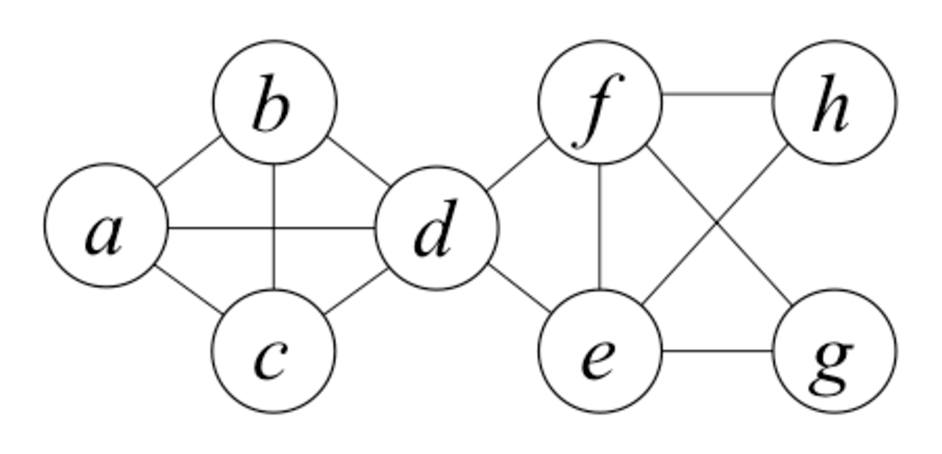
\includegraphics[scale=0.5]{./clique2g_1.eps}
\caption{4つの極大クリーク
\{$a,b,c,d$\}
\{$d,e,f$\}
\{$e,f,g$\}
\{$e,f,h$\}
が含まれる。
\label{fig:clique2g_1}}
\end{center}
\end{figure} 

\begin{figure}[htbp]
\begin{center}
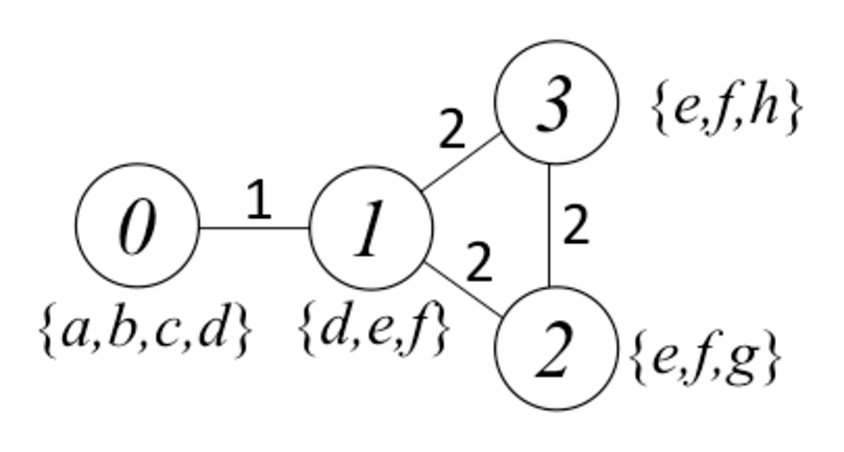
\includegraphics[scale=0.5]{./clique2g_2.eps}
\caption{新たに生成される極大クリークグラフ\label{fig:clique2g_2}}
\end{center}
\end{figure} 

さて、本コマンドの入力データであるオリジナルグラフは、表\ref{tbl:clique2g_1}に示されるような、
クリークIDと節点の2項目から構成されるCSV形式データである。
このデータは\ref{sect:mclique}節で示したmclique.rbコマンドで\verb|-node|を指定して出力されたデータに対応している。

そして、出力結果である極大クリークグラフは、節点データ(表\ref{tbl:clique2g_2})と枝データ(表\ref{tbl:clique2g_3})を別々に出力する。
節点データにおける\verb|weight|項目は、極大クリークを構成する節点数である。
また枝データにおける\verb|weight|項目は、極大クリークを構成する節点数である。

\begin{table}[htbp]
\begin{center}
\begin{tabular}{ccc}

\begin{minipage}{0.3\hsize}
\begin{center}
\caption{オリジナルグラフ\label{tbl:clique2g_1}}
{\small
\begin{tabular}{cc}
\hline
id&node \\
\hline
0&a \\
0&b \\
0&c \\
0&d \\
1&d \\
1&e \\
1&f \\
2&e \\
2&f \\
2&g \\
3&e \\
3&f \\
3&h \\
\hline
\end{tabular} 
}
\end{center}
\end{minipage}

\begin{minipage}{0.3\hsize}
\begin{center}
\caption{極大クリークグラフ(節点データ)\label{tbl:clique2g_2}}
{\small
\begin{tabular}{cccc}
\hline
node&weight \\
\hline
0&4 \\
1&3 \\
2&3 \\
3&3 \\
\hline
\end{tabular} 
}
\end{center}
\end{minipage}

\begin{minipage}{0.3\hsize}
\begin{center}
\caption{極大クリークグラフ(枝データ)\label{tbl:clique2g_3}}
{\small
\begin{tabular}{cccc}
\hline
node1&node2&weight \\
\hline
0&1&1 \\
1&2&2 \\
1&3&2 \\
2&3&2 \\
\hline
\end{tabular} 
}
\end{center}
\end{minipage}


\end{tabular} 
\end{center}
\end{table} 


\subsection{書式}
\begin{verbatim}
書式) mclique2g.rb i= [id=] [f=] eo= no= [T=] [--help]

  ファイル名指定
  i=  : クリークファイル名
	id= : クリークID項目名(デフォルト:"id")
  f=  : クリークを構成する節点項目名(デフォルト:"node")
  eo= : 出力枝ファイル名
  no= : 出力節点ファイル名

  その他
  T= : ワークディレクトリ(default:/tmp)
  --help : ヘルプの表示
\end{verbatim}

\subsection{利用例}
\subsubsection*{例1: 基本例}

前節で解説した例。


\begin{Verbatim}[baselinestretch=0.7,frame=single]
$ more clique.csv
id,node
0,a
0,b
0,c
0,d
1,d
1,e
1,f
2,e
2,f
2,g
3,e
3,f
3,h
$ mclique2g.rb i=clique.csv eo=edge.csv no=node.csv id=id f=node
#END# /usr/bin/mclique2g.rb i=clique.csv eo=edge.csv no=node.csv id=id f=node
$ more edge.csv
node1,node2,weight
0,1,1
1,2,2
1,3,2
2,3,2
$ more node.csv
node,weight
0,4
1,3
2,3
3,3
\end{Verbatim}




\section{mbiclique.rb 極大二部クリークの列挙\label{sect:mbiclique}}

本コマンドは、二部グラフから極大二部クリークを列挙する。
内部では\cite{UnoWeb}の\verb|lcm|コマンドを利用している。

$G=(V_1 \cup V_2,E)$を2つの部$V_1,V_2$の節点集合と部間の枝に張られた枝集合$E\subset V_1\times V_2$を持つ無向二部グラフとすると、
$V_1,V_2$の部分集合によって誘導される部分グラフの部間の任意の節点に枝があるような$G$の誘導部分グラフを二部クリークと呼ぶ。
%$V$の部分集合$V'$に対して$V'$によって誘導される部分グラフ$G'=(V',E(V'))(E'=\{(u,v) \in E|u,v \in V'\}$が完全グラフとなっている$G$の誘導部分グラフをクリークとい>う。
また、ある二部クリークが他の二部クリークの真部分集合でなければ、それは極大二部クリークと呼ばれる(図\ref{fig:biclique})。

\begin{figure}[htbp]
\begin{center}
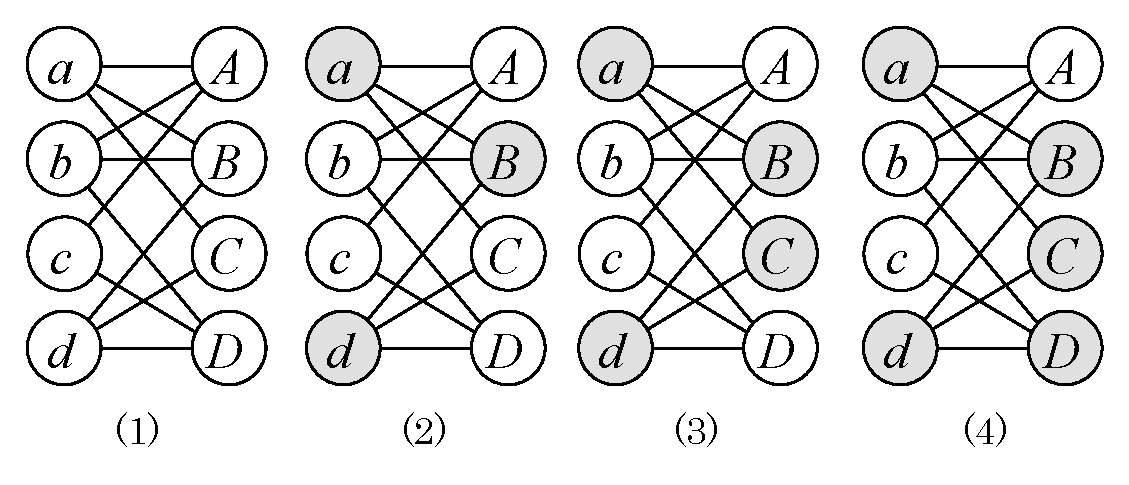
\includegraphics[scale=0.5]{./biclique.eps}
\caption{二部グラフ(1)について、網掛けで示された部分グラフ(2)は二部クリークではあるが、
(3)に示された二部クリークの真部分集合なので極大二部クリークではない。
一方で(3)はその他のどの二部クリークの真部分集合にはならないので極大である。
(4)は$a,D$間に枝がないので二部クリークではない。
\label{fig:biclique}}
\end{center}
\end{figure} 

極大二部クリークの列挙を使った応用例は多数考えられる。
例えば、消費者の食品購入パネルデータにおいて、一つの部を商品集合、他方の部を店集合と見なし、
ある閾値以上の購買のあった商品-店間に枝を張った二部グラフを構成できる。
そこから極大二部クリークを列挙することで、互いに強い関係にある商品と店のグルーピングが可能となる。

またテキストマイニングにおいては、格助詞句と用言句を各部と見なし、
用例のある格助詞句-用言句の間に枝を張った二部グラフを構成できる。
そこから極大二部クリークを列挙することで、互いに強い関係にある格フレーム(格助詞句-用言句ペアのこと)
のグルーピングが可能となり、ある種の概念を取得できる。

さらに、入札データにおいては、入札業者と案件をそれぞれ各部として考え、
実際に入札があった入札業者-案件の間に枝を張ることで二部グラフが構成できよう。

さて、本コマンドの入力データである二部グラフは、表\ref{tbl:bicl_input}に示されるような、
枝データを節点ペアとして表したCSV形式で与える(図\ref{fig:biclique} (1)に対応)。
項目が部を表している。
表\ref{tbl:bicl_input}では、小文字のアルファベットを要素として持つ\verb|node1|項目が一方の部を表し、
大文字のアルファベットを要素として持つ\verb|node2|項目が他方の部を表している。
グラフは無向グラフとして扱われ、島が複数あってもよい。

この二部グラフから極大二部クリークを列挙すると表\ref{tbl:bicl_output}に示されるような形式で
出力される。
一行が極大二部クリークに対応しており、各部を構成する要素が\verb|node1,node2|項目にベクトル形式で出力される。
\verb|size1,size2|には各部のサイズ(節点の数)が出力される。
5行目の極大二部クリーク($V_1=\{a,d\},V_2=\{B,C\}$)が図\ref{fig:biclique}(3)に対応している。
%また\verb|-node|オプションを指定することで
%\verb|node1,node2|項目にがクリークのIDで、この項目が同じ行で一つのクリークが識別される。
%\verb|id|=2のクリークが図\ref{fig:clique}(4)に対応し、
%\verb|id|=3のクリークが図\ref{fig:clique}(3)に対応している。
%その他にも、2つの節点から構成される極大クリーク$\{e,f\}$と$\{b,f\}$も列挙されている。
%最後の\verb|size|項目は、極大クリークを構成する節点数である。

\begin{table}[htbp]
\begin{center}
\begin{tabular}{cc}

\begin{minipage}{0.3\hsize}
\begin{center}
\caption{入力データ(枝データ)\label{tbl:bicl_input}}
{\small
\begin{tabular}{cc}
\hline
node1&node2 \\
\hline
a&A \\
a&B \\
a&C \\
b&A \\
b&B \\
b&D \\
c&A \\
c&D \\
d&B \\
d&C \\
d&D \\
\hline
\end{tabular} 
}
\end{center}
\end{minipage}

\begin{minipage}{0.3\hsize}
\begin{center}
\caption{出力結果\label{tbl:bicl_output}}
{\small
\begin{tabular}{llcc}
\hline
node1&node2&size1&size2 \\
\hline
a&A B C&1&3 \\
a b&A B&2&2 \\
a b c&A&3&1 \\
a b d&B&3&1 \\
a d&B C&2&2 \\
b&A B D&1&3 \\
b c&A D&2&2 \\
b c d&D&3&1 \\
b d&B D&2&2 \\
d&B C D&1&3 \\
\hline
\end{tabular} 
}
\end{center}
\end{minipage}

\end{tabular} 
\end{center}
\end{table} 

\subsection{書式}
\begin{verbatim}
書式) mbiclique.rb ei= ef= [o=] [l=] [u=] [T=] [-debug] [--help]

  ファイル名指定
  ei= : 辺データファイル
  ef= : 辺データ上の2つの節点項目名
  o=  : 出力ファイル
  l=  : 極大二部クリークを構成する最小節点数
      : ここで指定したサイズより小さい極大二部クリークは列挙されない。
      : カンマで区切って2つの値を指定すると、各部のサイズを制限できる。
      : カンマで区切った値の順番はef=で指定した項目の順番と同じ。
      : 制限を設けない場合は"l=2,"や"l=,2"のようにnull文字を指定する。
      : 後ろのnullは省略できる("l=2,"と"l=2"は同じ意味)。
  u=  : 極大二部クリークを構成する最大節点数
      : 指定の詳細はl=と同様である。

  その他
  T= : ワークディレクトリ(default:/tmp)
  --help : ヘルプの表示
\end{verbatim}

\subsection{注意点}
本コマンドの二部クリークの出力形式がベクトル形式(文字列を空白で区切った一つのCSV項目)となるため、
時に、一つの項目の長さが非常に長くなることがある。
そのため、内部で使っているMコマンドのCSV一行の最大長制約を超えてしまいエラーとなることがある。
そのようなときは、\verb|l=|もしくは\verb|u=|によって二部クリークのサイズを制約することで回避する。

\subsection{利用例}
\subsubsection*{Example 1: Basic Example}

Example illustrated from the previous section.


\begin{Verbatim}[baselinestretch=0.7,frame=single]
$ more dat.csv
node1,node2
a,A
a,B
a,C
b,A
b,B
b,D
c,A
c,D
d,B
d,C
d,D
$ mbiclique.rb i=dat.csv f=node1,node2 o=result1.csv
#MSG# converting paired form into transaction form ...
#MSG# lcm_20140215 CIf /tmp/__MTEMP_20452_70343276945380_0 1 /tmp/__MTEMP_20452_7034327694
5380_3
trsact: /tmp/__MTEMP_20452_70343276945380_0 ,#transactions 4 ,#items 4 ,size 11 extracted 
database: #transactions 4 ,#items 4 ,size 11
 output to: /tmp/__MTEMP_20452_70343276945380_3
separated at 0
iters=11
11
1
3
4
3
#END# /Users/stephane/.rvm/rubies/ruby-1.9.3-p448/bin/mbiclique.rb i=dat.csv f=node1,node2
 o=result1.csv
$ more result1.csv
node1,node2,size1,size2
a,A B C,1,3
a b,A B,2,2
a b c,A,3,1
a b d,B,3,1
a d,B C,2,2
b,A B D,1,3
b c,A D,2,2
b c d,D,3,1
b d,B D,2,2
d,B C D,1,3
\end{Verbatim}
\subsubsection*{Example 2: Example with size limit}

Enumerate maximal bipartite clique with size of 2 in columns \verb|node1,node2|.


\begin{Verbatim}[baselinestretch=0.7,frame=single]
$ mbiclique.rb i=dat.csv f=node1,node2 o=result2.csv l=2,2 u=2,2
#MSG# converting paired form into transaction form ...
#MSG# lcm_20140215 CIf -l 2 -u 2 /tmp/__MTEMP_20505_70100128947220_0 1 /tmp/__MTEMP_20505_
70100128947220_3
trsact: /tmp/__MTEMP_20505_70100128947220_0 ,#transactions 4 ,#items 4 ,size 11 extracted 
database: #transactions 4 ,#items 4 ,size 11
 output to: /tmp/__MTEMP_20505_70100128947220_3
separated at 0
iters=10
4
0
0
4
#END# /Users/stephane/.rvm/rubies/ruby-1.9.3-p448/bin/mbiclique.rb i=dat.csv f=node1,node2
 o=result2.csv l=2,2 u=2,2
$ more result2.csv
node1,node2,size1,size2
a b,A B,2,2
a d,B C,2,2
b c,A D,2,2
b d,B D,2,2
\end{Verbatim}
\subsubsection*{Example 3: Example to limit the partial size}

Enumerate maximal bipartite clique where column \verb|node1| with lower limit of 1 (Since the default lower limit is 1, this example does not reflect additional meaning),
and column \verb|node2| has a upper limit of 3.
The first value at \verb|u=| parameter is null, since the upper limit of column \verb|node1|. 


\begin{Verbatim}[baselinestretch=0.7,frame=single]
$ mbiclique.rb i=dat.csv f=node1,node2 o=result3.csv l=1, u=,3
#MSG# converting paired form into transaction form ...
#MSG# lcm_20140215 CIf -u 3 /tmp/__MTEMP_20558_70109238975520_0 1 /tmp/__MTEMP_20558_70109
238975520_3
trsact: /tmp/__MTEMP_20558_70109238975520_0 ,#transactions 4 ,#items 4 ,size 11 extracted 
database: #transactions 4 ,#items 4 ,size 11
 output to: /tmp/__MTEMP_20558_70109238975520_3
separated at 0
iters=11
11
1
3
4
3
#END# /Users/stephane/.rvm/rubies/ruby-1.9.3-p448/bin/mbiclique.rb i=dat.csv f=node1,node2
 o=result3.csv l=1, u=,3
$ more result3.csv
node1,node2,size1,size2
a,A B C,1,3
a b,A B,2,2
a b c,A,3,1
a b d,B,3,1
a d,B C,2,2
b,A B D,1,3
b c,A D,2,2
b c d,D,3,1
b d,B D,2,2
d,B C D,1,3
\end{Verbatim}




\section{mgdiff.rb - Graph Difference\label{sect:mgdiff}}

This command returns the difference between two general graph. 
However, as of this version, this command can be used to compare presence and absence of edge in undirected graph.  

\subsection{Format}
\begin{verbatim}
Format) mgdiff.rb i= f= m= [F=] [o=] [T=] [--help]

  Specify File Name 
  i= : File name of graph in edge data (node pair)
  f= : Field name of the 2 nodes in edge data
  m= : File name of reference graph (return the difference with this graph)
  F= : Field name of 2 nodes connected to the edge  in the reference file  (this parameter is not required if it is the same as f=)
  o= : Output file name
       Output the edge (node pair) from graph 1 data and graph 2 data based on the following values.  
        Field name: content
        i    :  file name specified at i=  if there is connected pair in the row 
       m    : file name specified at m= if there is connected pair in the row 
        diff : Classification of state
                1: only exist in graph specified at i=
                0: exist in graph in both i=,m=
               -1: only exist in graph specified at m=
  T= : Working directory (default:/tmp)
  --help : Help information
\end{verbatim}

\subsection{Examples}
\subsubsection*{例1: 基本例}



\begin{Verbatim}[baselinestretch=0.7,frame=single]
$ more g1.csv
node1,node2
a,b
b,c
c,d
$ more g2.csv
node1,node2
b,a
c,d
d,e
$ mgdiff.rb ei=g1.csv eI=g2.csv eo=result1.csv ef=node1,node2
#END# /usr/bin/mgdiff.rb ei=g1.csv eI=g2.csv eo=result1.csv ef=node1,node2
$ more result1.csv
node1,node2,ei,eI,diff
a,b,g1.csv,g2.csv,0
b,c,g1.csv,,1
c,d,g1.csv,g2.csv,0
d,e,,g2.csv,-1
\end{Verbatim}
\subsubsection*{例2: 有向グラフとしての比較}



\begin{Verbatim}[baselinestretch=0.7,frame=single]
$ mgdiff.rb ei=g1.csv eI=g2.csv eo=result2.csv ef=node1,node2 -dir
#END# /usr/bin/mgdiff.rb ei=g1.csv eI=g2.csv eo=result2.csv ef=node1,node2 -dir
$ more result2.csv
node1,node2,ei,eI,diff
a,b,g1.csv,,1
b,a,,g2.csv,-1
b,c,g1.csv,,1
c,d,g1.csv,g2.csv,0
d,e,,g2.csv,-1
\end{Verbatim}





\section{mcliqueInfo.rb 列挙されたクリークの各種情報\label{sect:mcliqueInfo}}

mclique.rbコマンドで列挙されたクリークについての各種情報を出力する。
本コマンドの主な目的は、クリーク同士の接続関係についての各種情報を出力することにある。

mclique2g.rbコマンドの解説で用いたグラフを図\ref{fig:mcinfo_1}に再掲する。
このグラフから得られる極大クリークは4つ存在する。
これら4つのクリークそれぞれについて、表\ref{tbl:mcinfo_1}に示す5つの情報を出力する。

\begin{table}[htbp]
\begin{center}
\caption{本コマンドの出力結果\label{tbl:mcinfo_1}}
%{\small
\begin{tabular}{lll}
\hline
出力項目名&内容&id=1(\{$d,e,f$\}の例) \\
\hline
nSize      & 節点数                    & 3 (節点$d,e,f$の3つ)\\
eSize      & 枝数(nSize$*$(nSize-1)/2) & 3 $(3*2/2=3)$\\
extNodes   & 外部接続節点数            & 5 (図\ref{fig:mcinfo_3}右) \\
extEdges   & 外部接続枝数              & 7 (図\ref{fig:mcinfo_3}左) \\
extCliques & 外部接続クリーク数        & 3 (図\ref{fig:mcinfo_2}) \\
\hline
\end{tabular} 
\end{center}
\end{table}


\begin{figure}[htbp]
\begin{center}
\begin{tabular}{cc}

\begin{minipage}{0.5\hsize}
\begin{center}
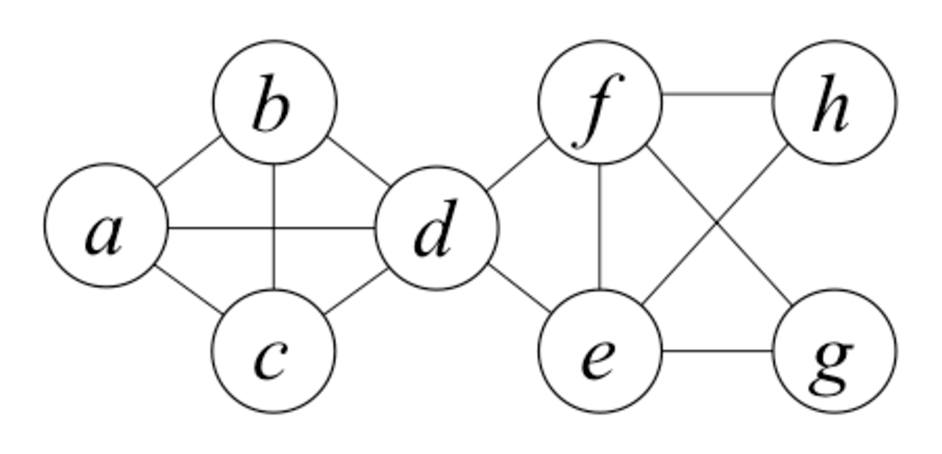
\includegraphics[scale=0.3]{./mcinfo_1.eps}
\caption{極大クリーク列挙の対象となるグラフ。
4つの極大クリーク\{a,b,c,d\}(id=0)、\{d,e,f\}(id=1)、\{e,f,g\}(id=2)、\{e,f,h\}(id=3)を含んでいる。\label{fig:mcinfo_1}}
\end{center}
\end{minipage}

\begin{minipage}{0.5\hsize}
\begin{center}
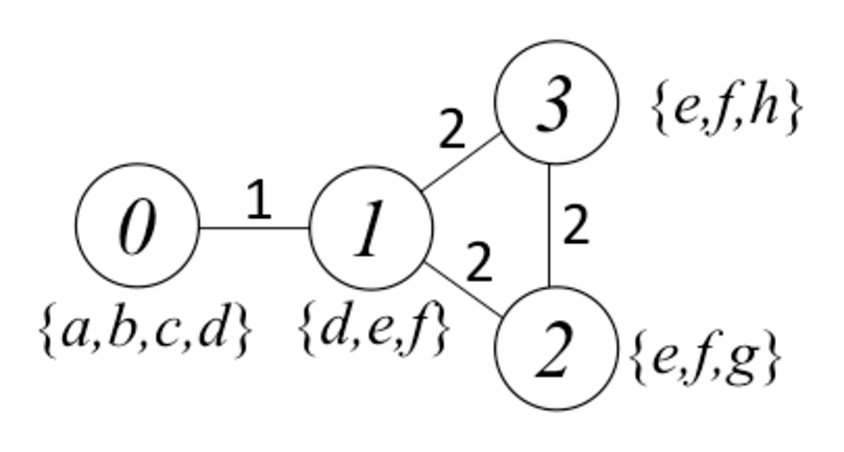
\includegraphics[scale=0.3]{./mcinfo_2.eps}
\caption{極大クリークグラフ。図\ref{fig:mcinfo_1}のクリークidを節点としたグラフ。
枝は共通の節点数を表している。
id=1のクリークは3つのクリークに直接の接続があることがわかる。
なお、このグラフを出力したければ\ref{sect:mclique2g}節を参照のこと。
\label{fig:mcinfo_2}}
\end{center}
\end{minipage}

\end{tabular} 
\end{center}
\end{figure} 

\begin{figure}[htbp]
\begin{center}
\begin{tabular}{c}

\begin{minipage}{0.5\hsize}
\begin{center}
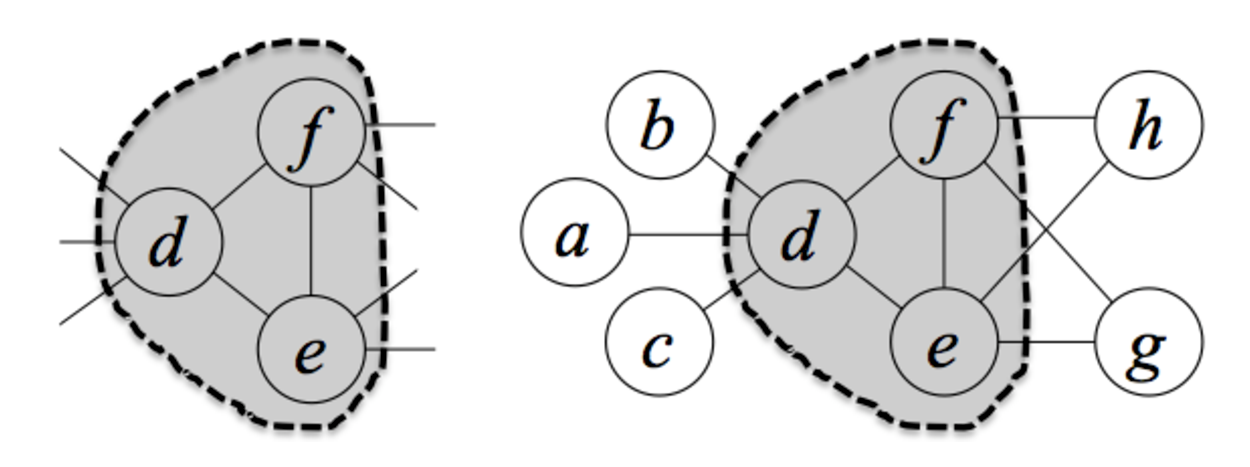
\includegraphics[scale=0.3]{./mcinfo_3.eps}
\caption{クリークid=1(グレーで示された領域)から外の節点へと接続される枝は7本ある(左図)。
クリークid=1(グレーで示された領域)から接続される節点数は5である(右図)。
\label{fig:mcinfo_3}}
\end{center}
\end{minipage}

\end{tabular} 
\end{center}
\end{figure} 

本コマンドの入力データは、\ref{sect:mclique2g}節に示したmclique2g.rbコマンド
と同様で、表\ref{tbl:clique2g_1}に示されるような、
クリークIDと節点の2項目から構成されるCSV形式データである。
そして、出力結果は、表\ref{tbl:mcinfo_3}に示されるように、
極大クリーク毎に表\ref{tbl:mcinfo_1}に示される情報が出力される。

\begin{table}[htbp]
\begin{center}
\begin{tabular}{cc}

\begin{minipage}{0.3\hsize}
\begin{center}
\caption{入力データ\label{tbl:mcinfo_2}}
{\small
\begin{tabular}{cc}
\hline
id&node \\
\hline
0&a \\
0&b \\
0&c \\
0&d \\
1&d \\
1&e \\
1&f \\
2&e \\
2&f \\
2&g \\
3&e \\
3&f \\
3&h \\
\hline
\end{tabular} 
}
\end{center}
\end{minipage}

\begin{minipage}{0.7\hsize}
\begin{center}
\caption{出力結果\label{tbl:mcinfo_3}}
{\small
\begin{tabular}{cccccc}
\hline
id&nSize&eSize&extNodes&extEdges&extCliques \\
\hline
0&4&6&2&2&1 \\
1&3&3&5&7&3 \\
2&3&3&2&4&2 \\
3&3&3&2&4&2 \\
\hline
\end{tabular} 
}
\end{center}
\end{minipage}

\end{tabular} 
\end{center}
\end{table} 



%これらのクリークと図に示された元のグラフとの関係について本コマンドは表\ref{tbl:ci_result}に示されるような結果を出力する。
%idはクリークを識別するIDで(図\ref{fig:ci_graph}のキャプションに記載)、それぞれのクリークについて表\ref{tbl:ci_flds}に示される情報を出力する。


\subsection{書式}
\begin{verbatim}
書式) mcliqueInfo.rb i= [id=] [f=] [m=] [F=] o= [T=] [--help]
  i=     : クリークデータファイル名
  id=    : クリークID項目名(デフォルト:"id")
  f=     : クリークを構成する節点項目名(デフォルト:"node")

  T= : ワークディレクトリ(default:/tmp)
  --help : ヘルプの表示
\end{verbatim}

\subsection{利用例}
\subsubsection*{例1: 基本例}

前節で解説した例。


\begin{Verbatim}[baselinestretch=0.7,frame=single]
$ more clique.csv
id,node
0,a
0,b
0,c
0,d
1,d
1,e
1,f
2,e
2,f
2,g
3,e
3,f
3,h
$ mcliqueInfo.rb i=clique.csv o=result1.csv id=id f=node
#END# /usr/bin/mcliqueInfo.rb i=clique.csv o=result1.csv id=id f=node
$ more result1.csv
id,nSize,eSize,extNodes,extEdges,extCliques
0,4,6,2,2,1
1,3,3,5,7,3
2,3,3,2,4,2
3,3,3,2,4,2
\end{Verbatim}




%\chapter{その他}

%\bibliographystyle{plain-annote}
%\bibliography{mybibliography}

\begin{thebibliography}{9}
\bibitem{Bishop2008}
C.M. ビショップ著, 元田浩, 栗田多喜夫, 樋口知之, 松本裕治, 村田昇(編), パターン認識と機械学習(下):ベイズ理論による統計的予測, 13章, pp.323--370, 2008.

\bibitem{Karypis1999}
Karypis, G. and Kumar, V., "A fast and high quality multilevel scheme for partitioning irregular graphs", SIAM Journal on Scientific Computing 20 (1), pp.359--392, 1999.

\bibitem{Karypis1998}
Karypis, G. and Kumar, V., "Multilevel k-way Partitioning Scheme for Irregular Graphs",
Journal of Parallel and Distributed Compupting 48, pp.96--129, 1998.

\bibitem{SSS94}
S. Shimozono, A. Shinohara, T. Shinohara, S. Miyano, S. Kuhara and S. Arikawa,
Knowledge Acquisition from Amino Acid Sequences by Machine Learning System
BONSAI, {\em Trans. Information Processing Society of Japan},
Vol. 35, pp. 2009-2018, 1994.

\bibitem{Quinlan93}
J. R. Quinlan, {\em C4.5: Programs for Machine Learning}, San Meteo: Morgan Kaufmann, 1993.

\bibitem{Breiman84}
L. Breiman, J. Friedman, R. Olshen, C. Stone
{\em  Classification and regression trees},
Wadsworth: Belmont, CA, 1984.

\end{thebibliography}




\end{document}
\end

